\mainchapter{Implementación}{\topbanner}\label{cap:implementacio}
\vspace*{0.7cm}

En esta sección se describe el proceso de implementación de la solución de servicio de directorio, partiendo del diseño definido en el capítulo anterior. Primero se presenta la metodología y el entorno utilizado para el despliegue. A continuación se detallan las etapas de instalación y configuración del servidor principal FreeIPA, seguidas de la instalación del servidor réplica y la configuración de HAProxy como punto de acceso unificado. Finalmente, se describe la integración de FreeIPA con los servicios OpenVPN, OpenProject y Xen Orchestra, incluyendo la verificación del funcionamiento de cada componente.

\section{Metodología}\label{sec:metodologia-implementacio}

Para el desarrollo de la fase de implementación se utilizó un servidor tipo torre perteneciente a la infraestructura del grupo de investigación \ac{GRID}, sobre el cual se desplegó el entorno destinado a la ejecución de la arquitectura definida durante la etapa de diseño. Este enfoque permitió disponer de una infraestructura controlada para llevar a cabo la instalación, configuración, integración y validación de cada uno de los componentes del sistema.

Con el propósito de aprovechar los recursos disponibles y mantener el aislamiento de los servicios, se implementó un esquema de virtualización mediante la creación de las máquinas virtuales correspondientes a cada uno de los elementos de la solución. Asimismo, se realizó la asignación de los recursos de procesamiento, memoria y almacenamiento de acuerdo con los requisitos particulares de cada servicio, considerando aspectos relacionados con el rendimiento, la disponibilidad y la escalabilidad de la infraestructura.

De manera complementaria, se efectuó la configuración del esquema de red definido para el proyecto, incluyendo el direccionamiento de los equipos, la resolución de nombres, la definición de los nombres de dominio completamente calificados (\ac{FQDN}), la sincronización horaria y la aplicación de las reglas de seguridad necesarias para permitir el funcionamiento de los servicios implementados.

Finalmente, se llevó a cabo el proceso de instalación y configuración de la plataforma FreeIPA y de los servicios asociados a esta, verificando la correcta integración entre los distintos componentes y el cumplimiento de los requisitos funcionales y de seguridad establecidos para la infraestructura del grupo de investigación \ac{GRID}.

\section{Instalación del servidor principal de FreeIPA}\label{sec:instalacion-servidor-principal}

Inicialmente, se llevó a cabo la creación de la máquina virtual destinada a alojar el servidor principal de la infraestructura. Sobre esta se instaló el sistema operativo Fedora Server 44, seleccionado de acuerdo con los requisitos y las recomendaciones de compatibilidad establecidas para la implementación de la plataforma FreeIPA. Asimismo, la máquina virtual se configuró de acuerdo con las especificaciones técnicas definidas durante la fase de diseño, considerando los recursos de procesamiento, memoria, almacenamiento y conectividad necesarios para el correcto funcionamiento del servicio implementado, como se muestra en la \autoref{fig:creacion-vm-ipa1}.

\begin{figure}[H]
	\centering
	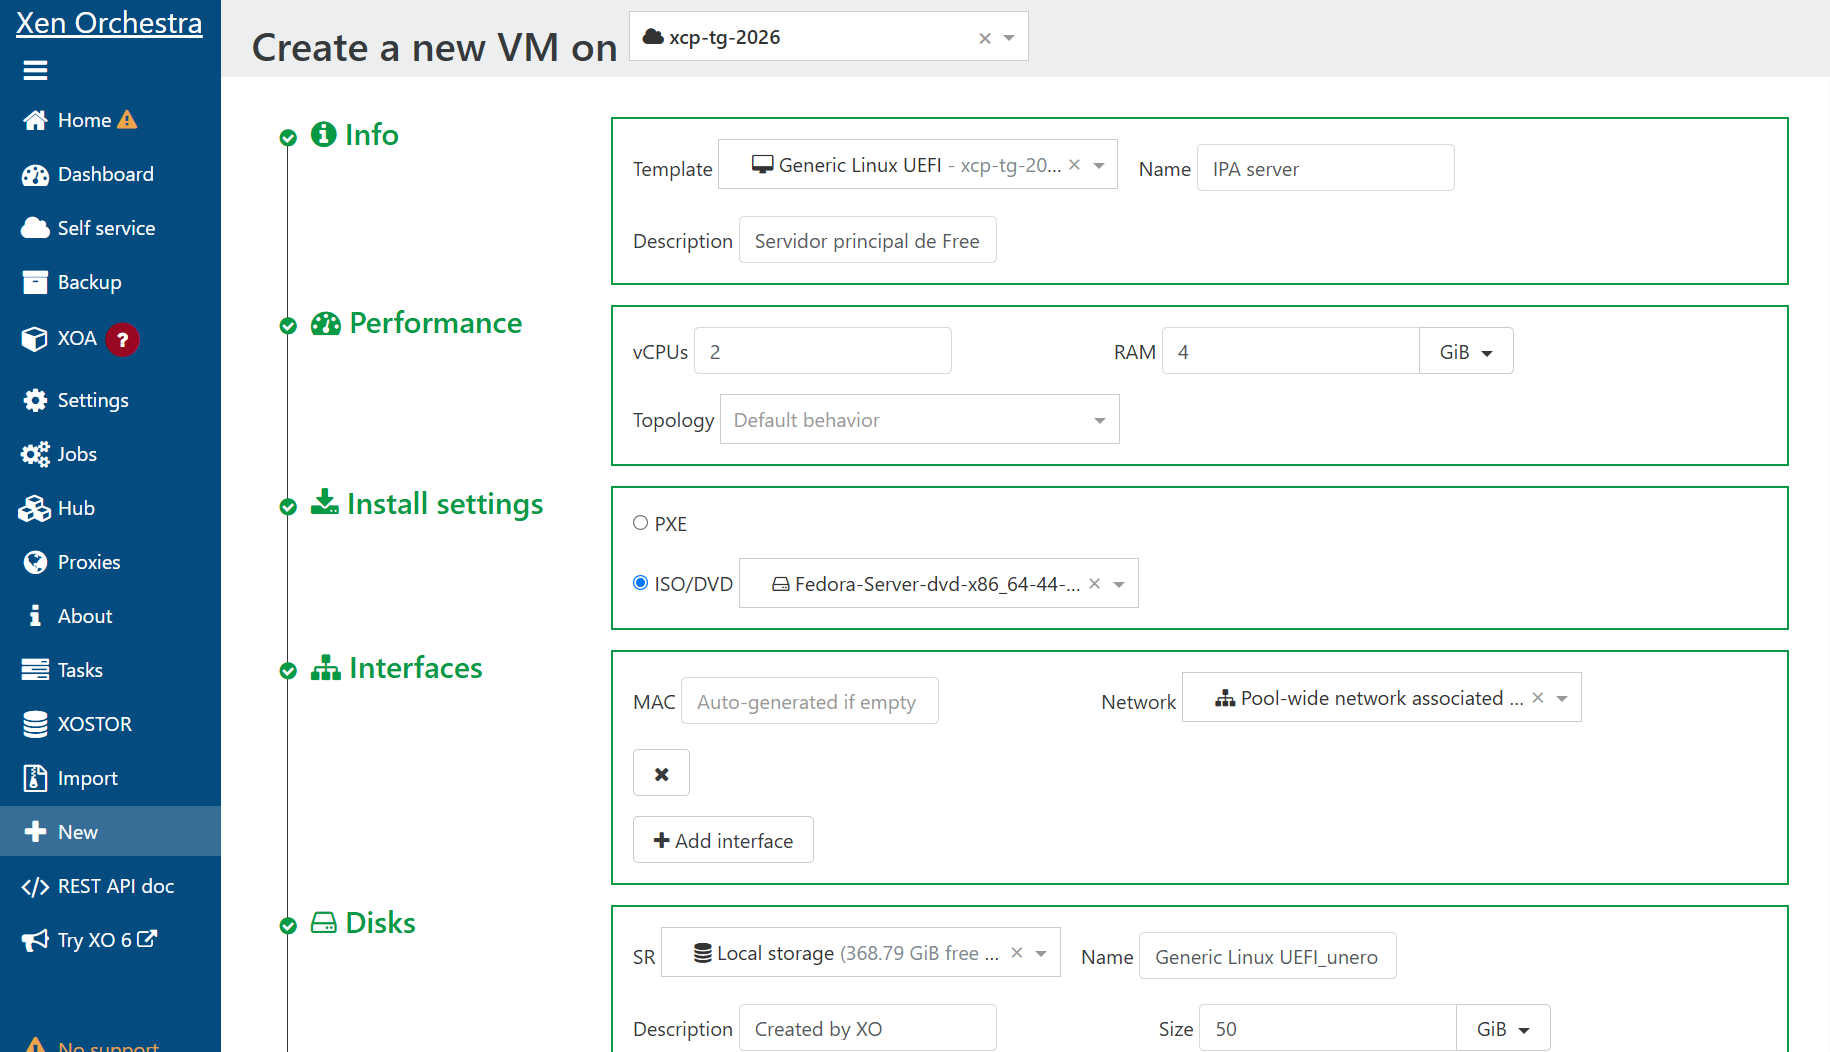
\includegraphics[width=0.9\textwidth]{mainmatter/II-desarrollo-metodologico/implementacion/imagenes/creacion-vm-ipa1.png}
	\caption{Creación de la máquina virtual del servidor principal}
	\label{fig:creacion-vm-ipa1}
\end{figure}

Posteriormente, se realizó la instalación del sistema operativo sobre la máquina virtual creada previamente, como se muestra en la \autoref{fig:instalacion-sistema-operativo}.

\begin{figure}[H]
	\centering
	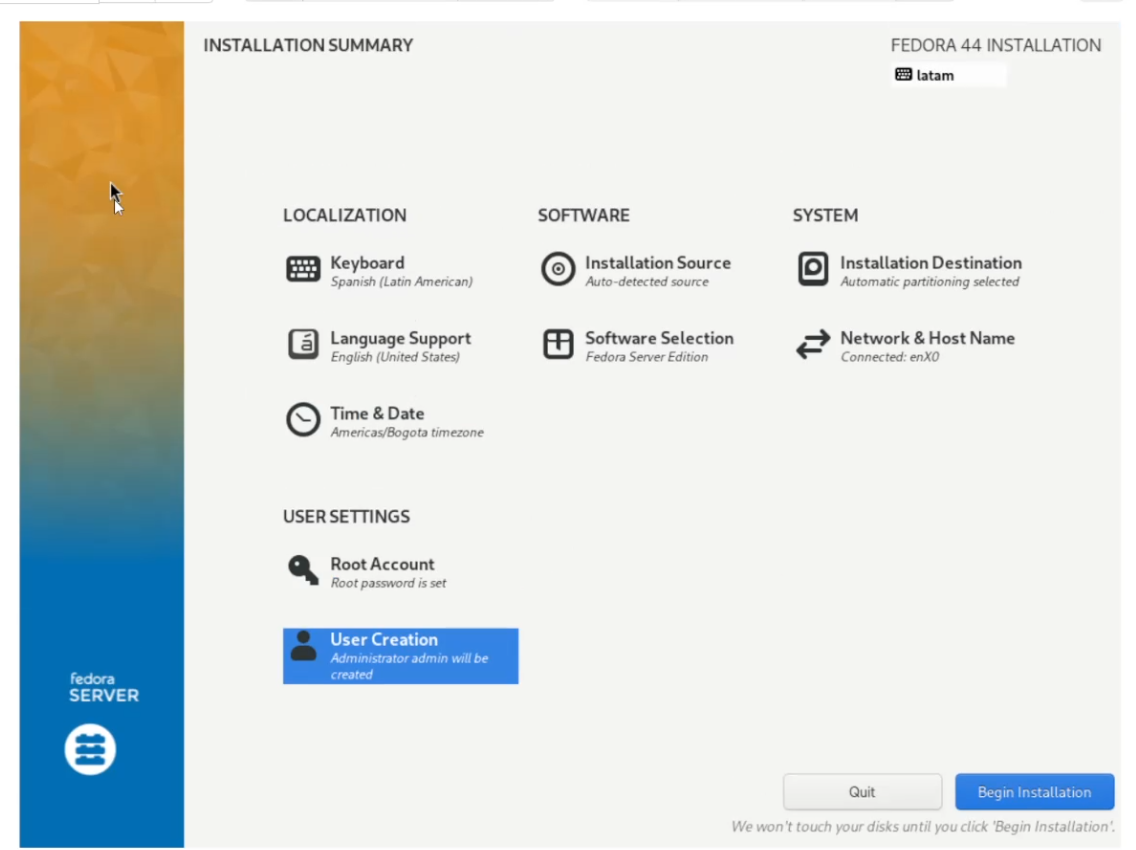
\includegraphics[width=0.9\textwidth]{mainmatter/II-desarrollo-metodologico/implementacion/imagenes/instalacion-sistema-operativo.png}
	\caption{Instalación del sistema operativo Fedora Server 44 en el servidor principal}
	\label{fig:instalacion-sistema-operativo}
\end{figure}

Como parte de la configuración inicial del sistema, se configuró la interfaz de red de la máquina virtual, asignándole la dirección \acs{IP} previamente definida dentro del esquema de direccionamiento de la infraestructura. Esta configuración garantiza la conectividad con los demás componentes del entorno y constituye un requisito indispensable para la instalación y configuración del servidor FreeIPA. En la \autoref{fig:configuracion-ip-ipa1} se observa la configuración de red realizada.

\begin{figure}[H]
	\centering
	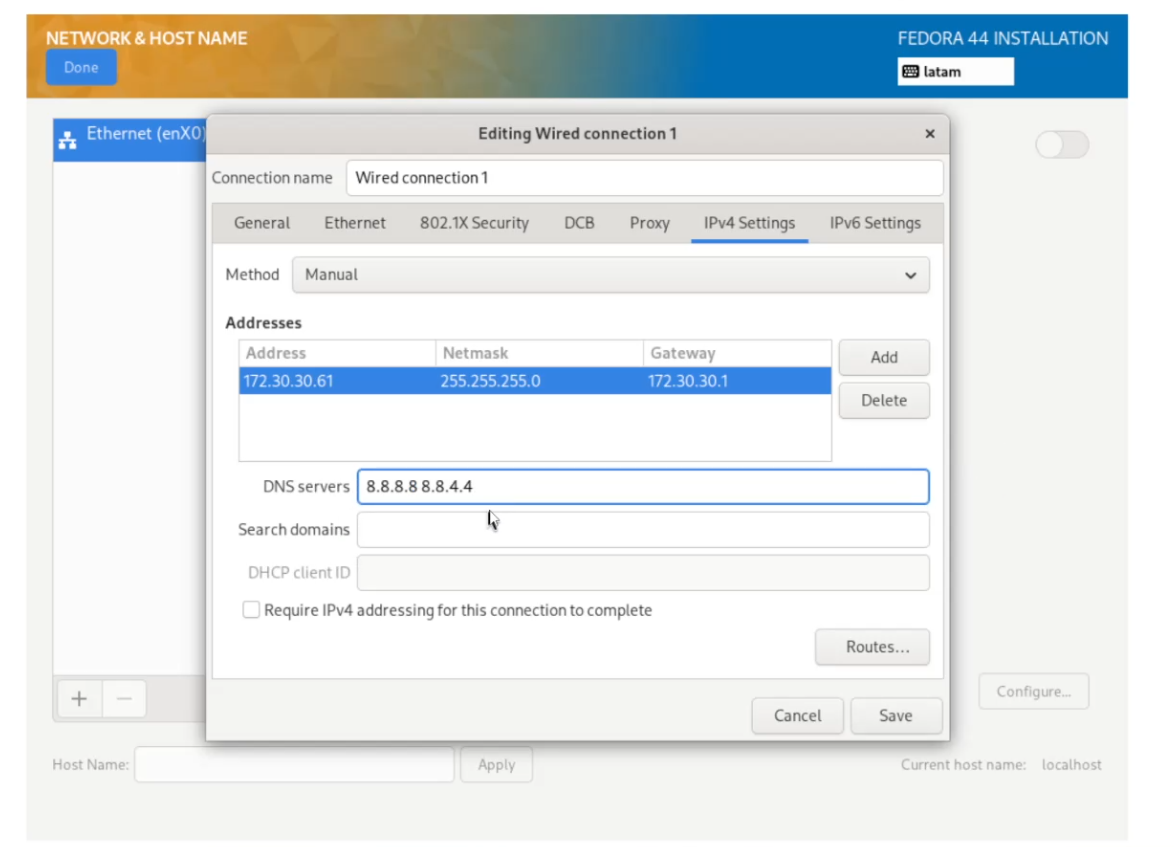
\includegraphics[width=0.9\textwidth]{mainmatter/II-desarrollo-metodologico/implementacion/imagenes/configuracion-ip-ipa1.png}
	\caption{Configuración de la interfaz de red de la máquina virtual}
	\label{fig:configuracion-ip-ipa1}
\end{figure}

Una vez finalizada la instalación del sistema operativo, se realizaron las configuraciones previas requeridas para la instalación de FreeIPA, siguiendo el procedimiento recomendado en la documentación oficial del proyecto. Como primer paso, se configuró el nombre de dominio completamente calificado (\acs{FQDN}) del servidor, utilizando el nombre \textbf{ipa1.grid.uniquindio.edu.co}, como se muestra en la \autoref{fig:nombre-host-ipa1}.

\begin{figure}[H]
	\centering
	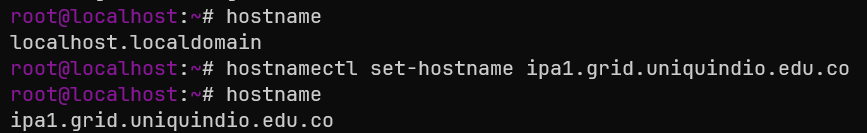
\includegraphics[width=0.9\textwidth]{mainmatter/II-desarrollo-metodologico/implementacion/imagenes/nombre-host-ipa1.png}
	\caption[Configuración del nombre de dominio]{Configuración del nombre de dominio completamente calificado del servidor principal de FreeIPA}
	\label{fig:nombre-host-ipa1}
\end{figure}

Posteriormente, se agregó la entrada correspondiente al servidor en el archivo \path{/etc/hosts}, asociando la dirección \acs{IP} \textbf{172.30.30.61} con el nombre de dominio \textbf{\nolinkurl{ipa.grid.uniquindio.edu.co}} y su nombre corto \textbf{ipa1}. Esta configuración permite la correcta resolución local del nombre del servidor, requisito necesario para el adecuado funcionamiento y la instalación de FreeIPA. El resultado de esta modificación se ilustra en la \autoref{fig:archivo-hosts-ipa1}.

\begin{figure}[H]
	\centering
	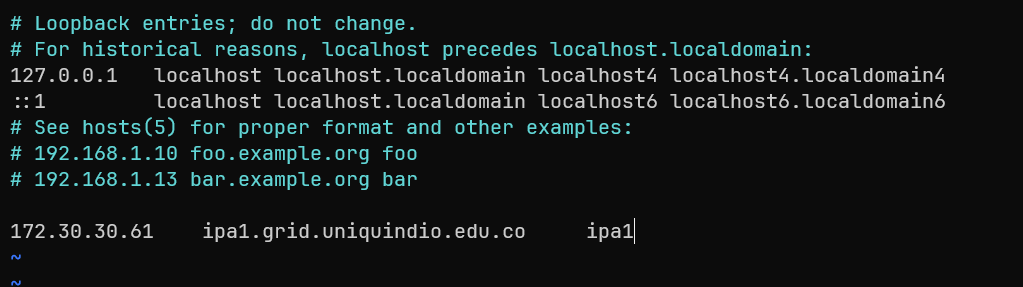
\includegraphics[width=0.9\textwidth]{mainmatter/II-desarrollo-metodologico/implementacion/imagenes/archivo-hosts-ipa1.png}
	\caption{Configuración del archivo /etc/hosts}
	\label{fig:archivo-hosts-ipa1}
\end{figure}

Posteriormente, se configuraron las reglas del cortafuegos necesarias para el funcionamiento del servidor FreeIPA. Para ello, se habilitaron de forma permanente los servicios correspondientes a \ac{LDAP} y \ac{LDAPS} y, a continuación, se recargó la configuración del cortafuegos con el fin de aplicar los cambios realizados.

Esta configuración permite que los diferentes componentes de la infraestructura puedan establecer comunicación con el servidor y garantiza la disponibilidad de los servicios requeridos para los procesos de autenticación y administración centralizada. En la \autoref{fig:reglas-cortafuegos-ipa1} se presenta el procedimiento realizado y el resultado obtenido tras la verificación de la configuración.

\begin{figure}[H]
	\centering
	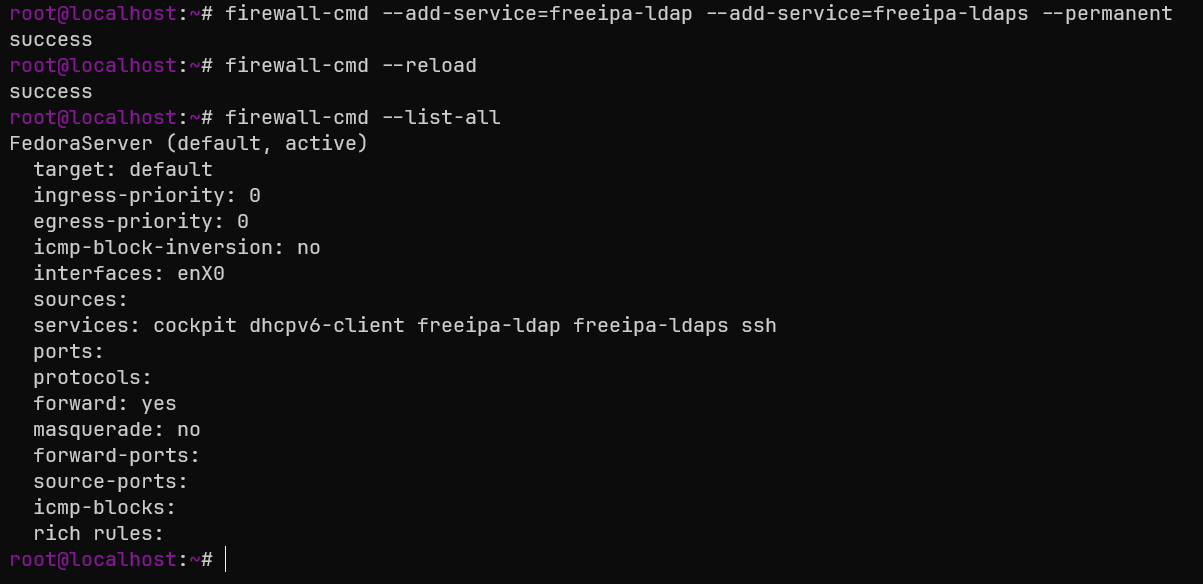
\includegraphics[width=0.9\textwidth]{mainmatter/II-desarrollo-metodologico/implementacion/imagenes/reglas-cortafuegos-ipa1.png}
	\caption{Configuración de las reglas del cortafuegos para los servicios de FreeIPA}
	\label{fig:reglas-cortafuegos-ipa1}
\end{figure}

Una vez completadas las configuraciones previas del sistema, se procedió a la instalación del paquete freeipa-server mediante el gestor de paquetes dnf, el cual contiene los componentes necesarios para el despliegue y la administración del servidor FreeIPA. En la \autoref{fig:instalacion-paquete-ipa1} se observa la ejecución de este procedimiento.

\begin{figure}[H]
	\centering
	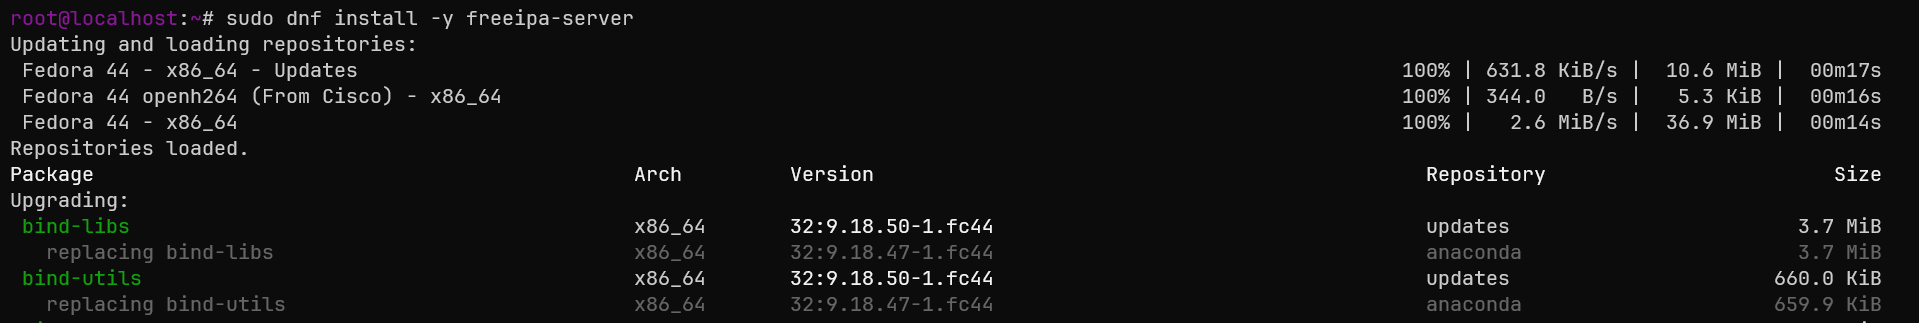
\includegraphics[width=0.8\textwidth]{mainmatter/II-desarrollo-metodologico/implementacion/imagenes/instalacion-paquete-ipa1.png}
	\caption{Instalación del paquete freeipa-server}
	\label{fig:instalacion-paquete-ipa1}
\end{figure}

Posteriormente, se ejecutó el comando ipa-server-install, el cual inicia el proceso de instalación y configuración de FreeIPA a través de un asistente interactivo. Debido a que el nombre de dominio completamente calificado (\ac{FQDN}) ya había sido definido previamente como ipa1.grid.uniquindio.edu.co, el instalador detectó automáticamente parte de la información requerida y propuso los valores predeterminados correspondientes.

Entre los parámetros configurados se encuentra el \ac{FQDN} \nolinkurl{ipa1.grid.uniquindio.edu.co}, utilizado para identificar de manera única el servidor dentro de la infraestructura. A partir de este valor se determinó el dominio grid.uniquindio.edu.co, mientras que el dominio de Kerberos (realm) se estableció como \nolinkurl{GRID.UNIQUINDIO.EDU.CO}, siguiendo la convención de utilizar letras mayúsculas para este tipo de identificadores.

Asimismo, se definieron las credenciales correspondientes al usuario Directory Manager, encargado de las tareas administrativas del servicio de directorios, y al usuario admin, utilizado para la administración de la plataforma FreeIPA. Del mismo modo, se configuró el nombre de NetBIOS \ac{GRID}, necesario para garantizar la compatibilidad con determinados servicios y mecanismos de interoperabilidad.

Por otra parte, el instalador detectó la dirección \acs{IP} 172.30.30.61, correspondiente al servidor principal, la cual fue utilizada como base para la configuración de red del servicio.

Finalmente, el asistente llevó a cabo la instalación y configuración de los distintos componentes de la plataforma, entre los que se encuentran 389 Directory Server, el Centro de Distribución de Claves de Kerberos (\acs{KDC}), la autoridad certificadora (\acs{CA}), el servidor web Apache y los servicios encargados de la gestión centralizada de identidades y certificados. Las \autoref{fig:instalacion-servidor-ipa1-paso-1} y \autoref{fig:instalacion-servidor-ipa1-paso-2} presentan el procedimiento de instalación y los parámetros definidos durante este proceso.

\begin{figure}[H]
	\centering
	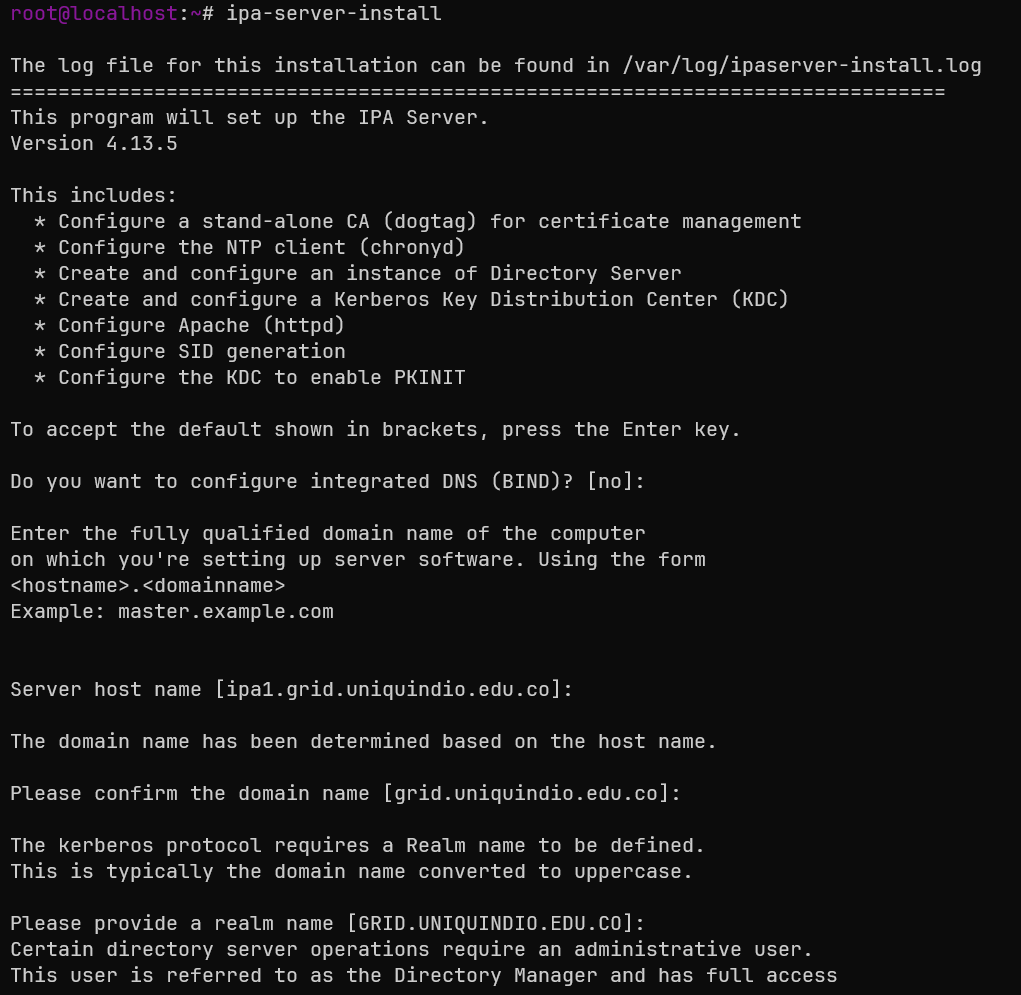
\includegraphics[width=0.6\textwidth]{mainmatter/II-desarrollo-metodologico/implementacion/imagenes/instalacion-servidor-ipa1-paso-1.png}
	\caption{Proceso de instalación y configuración inicial de FreeIPA parte 1}
	\label{fig:instalacion-servidor-ipa1-paso-1}
\end{figure}

\begin{figure}[H]
	\centering
	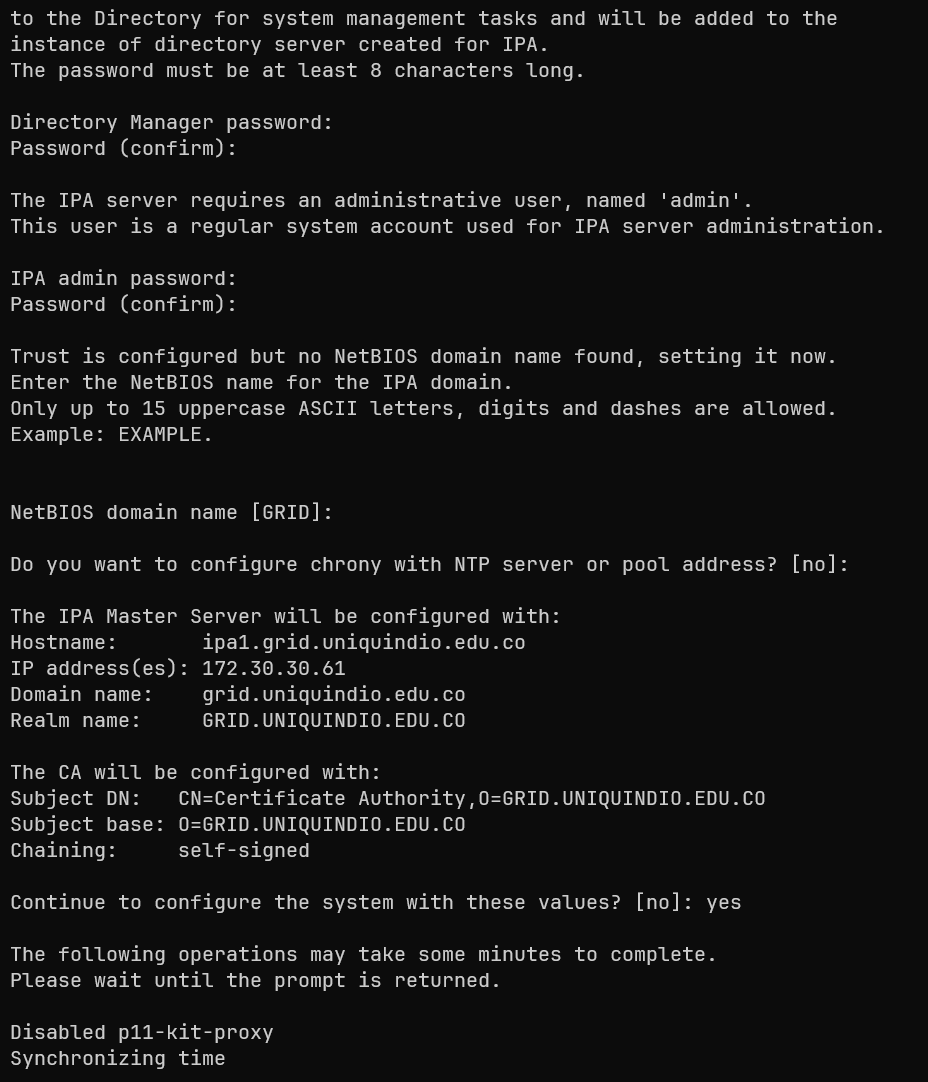
\includegraphics[width=0.6\textwidth]{mainmatter/II-desarrollo-metodologico/implementacion/imagenes/instalacion-servidor-ipa1-paso-2.png}
	\caption{Proceso de instalación y configuración inicial de FreeIPA parte 2}
	\label{fig:instalacion-servidor-ipa1-paso-2}
\end{figure}

\section{Configuración del servidor FreeIPA}\label{sec:configuracion-servidor-freeipa}

Una vez finalizada la instalación del servidor, se procedió a realizar la configuración inicial de la plataforma FreeIPA, incorporando los usuarios, grupos y políticas necesarios para el funcionamiento de la infraestructura y la integración de los servicios definidos durante la fase de diseño.

\subsection{Creación de grupos de usuarios}

Una vez finalizada la instalación de la plataforma, se procedió a la creación de los grupos de usuarios necesarios para la gestión del acceso a los servicios integrados en la infraestructura. Estos grupos constituyen el principal mecanismo de autorización, ya que permiten asociar a cada usuario los permisos correspondientes en función del servicio al que deba acceder.

En particular, se crearon los grupos openproject, openvpn y xenorchestra, destinados a controlar el acceso a OpenProject, OpenVPN y Xen Orchestra, respectivamente. Del mismo modo, se creó el grupo ldap-cuentas-servicio, empleado para administrar las cuentas de servicio utilizadas por las diferentes aplicaciones para establecer la comunicación con el directorio. Los grupos configurados en la plataforma se muestran en la \autoref{fig:grupos-usuarios}.

\begin{figure}[H]
	\centering
	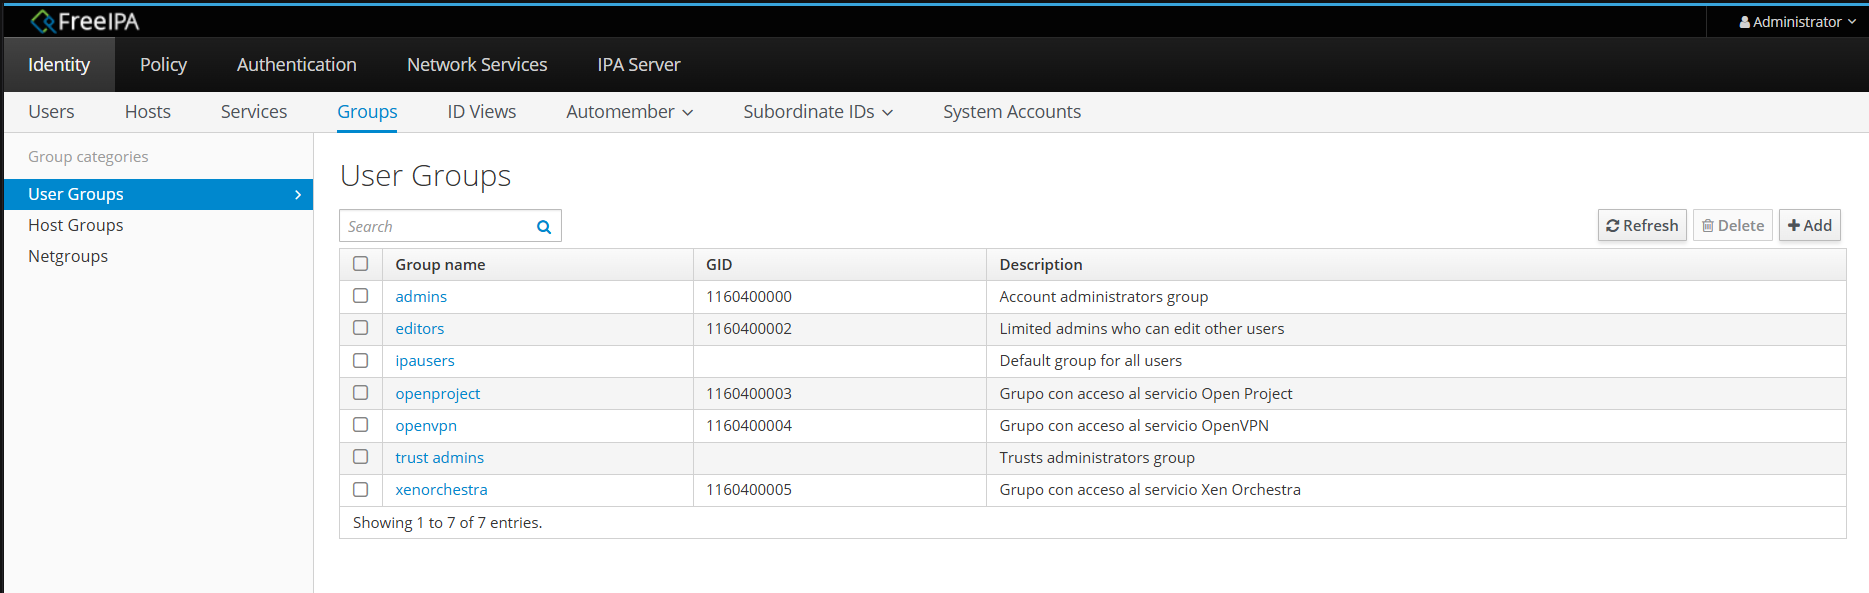
\includegraphics[width=0.8\textwidth]{mainmatter/II-desarrollo-metodologico/implementacion/imagenes/grupos-usuarios.png}
	\caption{Grupos de usuarios configurados en FreeIPA}
	\label{fig:grupos-usuarios}
\end{figure}

\subsection{Políticas de contraseñas}

Una vez creados los grupos de usuarios, se procedió a definir las políticas de contraseñas que regirán el funcionamiento de la plataforma. En primer lugar, se configuró la política global, la cual se aplica de forma predeterminada a todos los usuarios administrados por FreeIPA.

Con el objetivo de fortalecer la seguridad de la infraestructura, se estableció una vigencia máxima de ciento ochenta días para las contraseñas, un período mínimo de veinticuatro horas entre cambios consecutivos y un historial de cinco contraseñas para impedir la reutilización inmediata de credenciales. Asimismo, se definió una longitud mínima de doce caracteres y la obligatoriedad de emplear cuatro categorías de caracteres diferentes.

De igual manera, se limitó a cinco el número máximo de intentos fallidos de autenticación, se configuró un intervalo de sesenta segundos para el restablecimiento del contador de errores y se estableció un período de bloqueo de trescientos segundos. Finalmente, se permitió un máximo de tres inicios de sesión de gracia, los cuales permiten ingresar a los servicios después de vencida la contraseña, esto con el fin de facilitar el cambio de las credenciales una vez alcanzada la fecha de vencimiento. La configuración completa de esta política se presenta en la \autoref{fig:politica-contrasena-global}.

\begin{figure}[H]
	\centering
	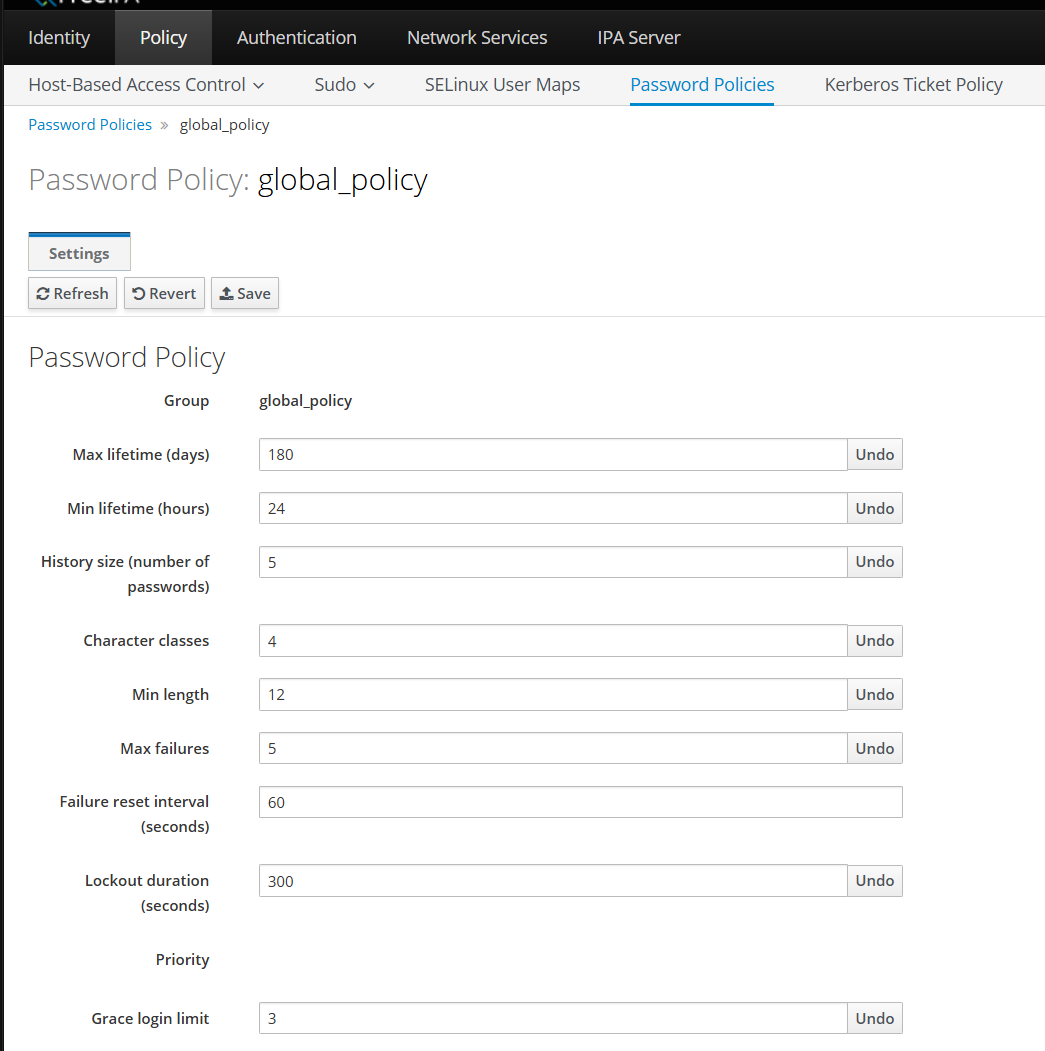
\includegraphics[width=0.8\textwidth]{mainmatter/II-desarrollo-metodologico/implementacion/imagenes/politica-contrasena-global.png}
	\caption{Configuración de la política global de contraseñas}
	\label{fig:politica-contrasena-global}
\end{figure}

Posteriormente, se creó una política específica para el grupo ldap-cuentas-servicio. El propósito de esta configuración fue impedir el vencimiento de las contraseñas asociadas a las cuentas de servicio, garantizando así la disponibilidad continua de los mecanismos de autenticación e integración empleados por las distintas plataformas conectadas al servicio de directorio. La política configurada se observa en la \autoref{fig:politica-contrasena-servicio}.

\begin{figure}[H]
	\centering
	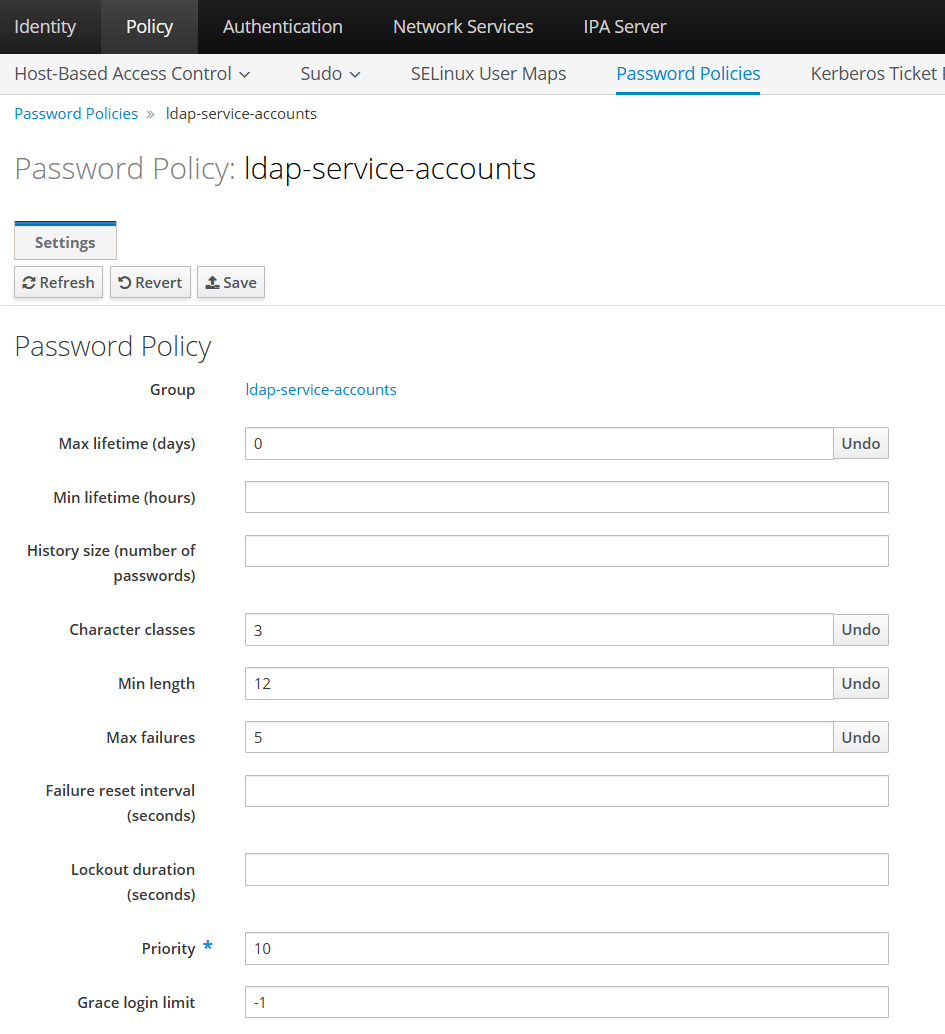
\includegraphics[width=0.8\textwidth]{mainmatter/II-desarrollo-metodologico/implementacion/imagenes/politica-contrasena-servicio.png}
	\caption{Política de contraseñas para las cuentas de servicio}
	\label{fig:politica-contrasena-servicio}
\end{figure}

\subsection{Creación de cuentas de servicio}

Posteriormente, se llevó a cabo la creación de las cuentas de servicio empleadas por las diferentes plataformas para establecer la comunicación con el servidor FreeIPA. Estas cuentas permiten que las aplicaciones realicen consultas al directorio y ejecuten los procesos de autenticación y autorización necesarios para su funcionamiento.

Con el fin de facilitar su administración y aplicar políticas específicas, todas las cuentas creadas fueron incorporadas al grupo ldap-cuentas-servicio. De esta manera, fue posible centralizar la gestión de sus permisos y garantizar la aplicación uniforme de las medidas de seguridad definidas para este tipo de cuentas. Las cuentas de servicio configuradas se presentan en la \autoref{fig:cuentas-servicio}.

\begin{figure}[H]
	\centering
	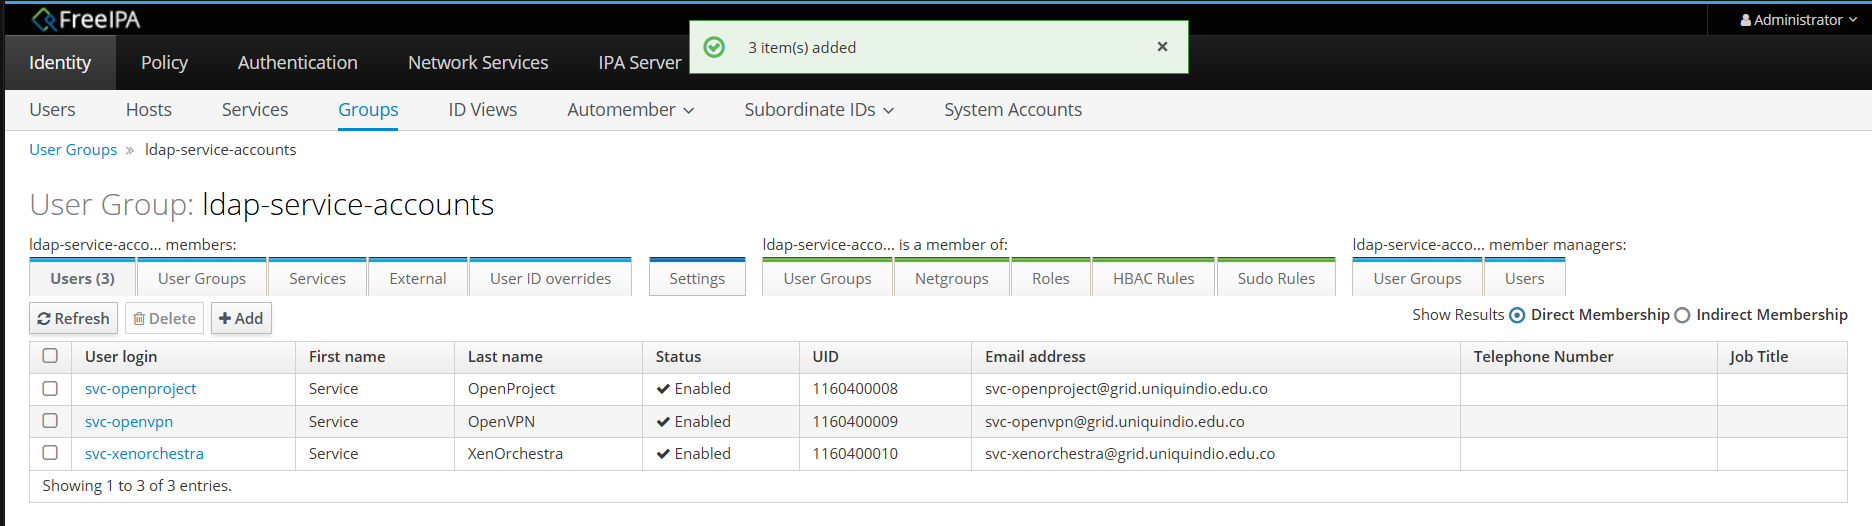
\includegraphics[width=0.8\textwidth]{mainmatter/II-desarrollo-metodologico/implementacion/imagenes/cuentas-servicio.png}
	\caption{Cuentas de servicio configuradas en FreeIPA}
	\label{fig:cuentas-servicio}
\end{figure}


\section{Instalación del servidor réplica de FreeIPA}\label{sec:instalacion-servidor-replica}

La creación de la máquina virtual destinada a alojar el servidor de réplica se realizó siguiendo el mismo procedimiento empleado para el servidor principal. En consecuencia, se utilizaron las mismas especificaciones de procesamiento, memoria y almacenamiento definidas durante la fase de diseño.

La principal diferencia con respecto a la configuración anterior correspondió a los parámetros de red, ya que fue necesario asignar una dirección \ac{IP} diferente para identificar de manera única el nuevo servidor dentro de la infraestructura. La configuración aplicada a la máquina virtual de la réplica se presenta en la \autoref{fig:configuracion-ip-ipa2}.

\begin{figure}[H]
	\centering
	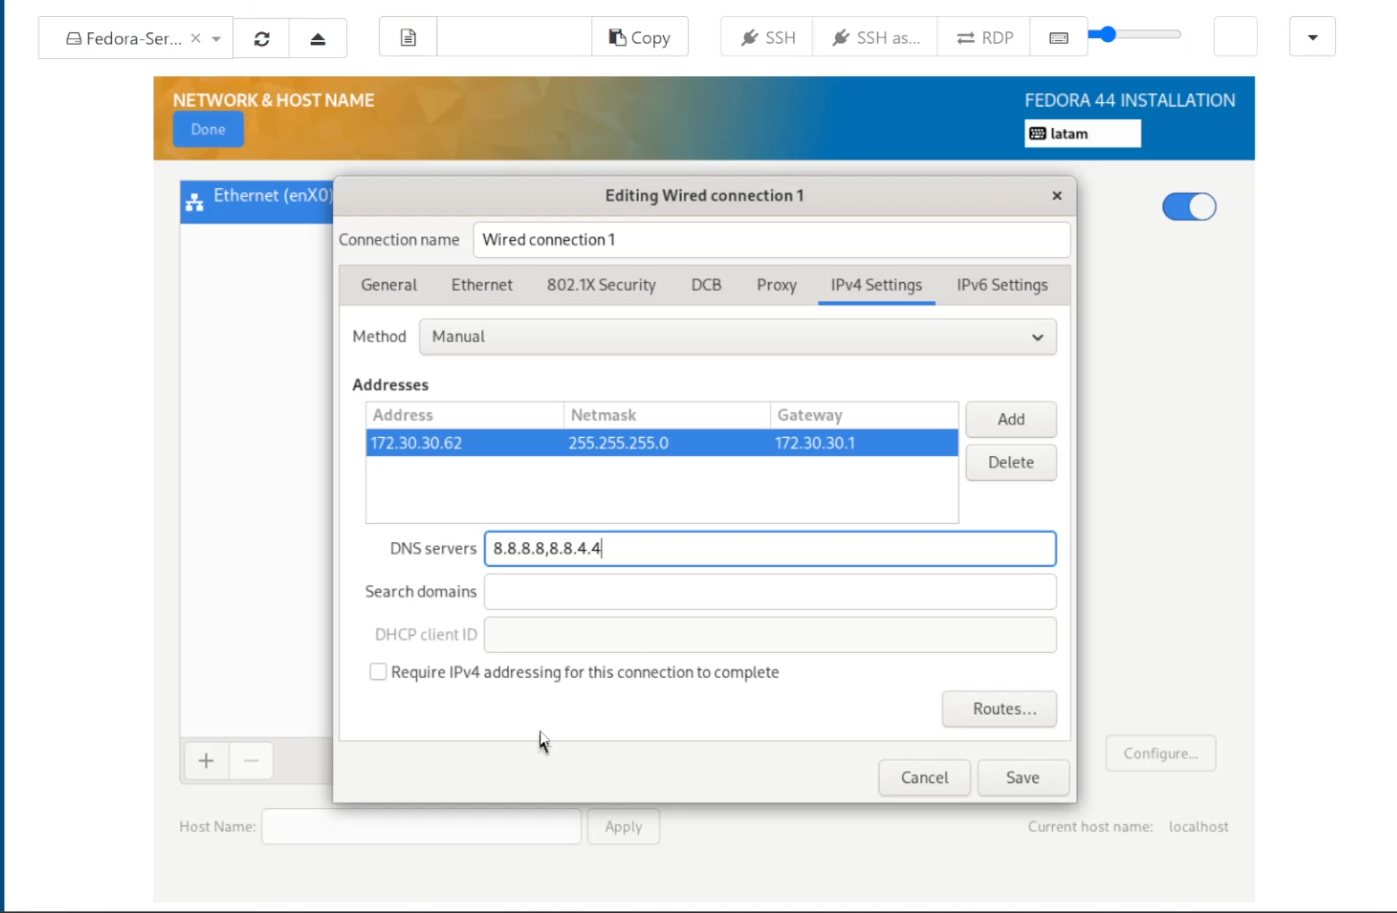
\includegraphics[width=0.8\textwidth]{mainmatter/II-desarrollo-metodologico/implementacion/imagenes/configuracion-ip-ipa2.png}
	\caption{Configuración de red del servidor de réplica}
	\label{fig:configuracion-ip-ipa2}
\end{figure}

Una vez creada la máquina virtual destinada al servidor de réplica y realizada la configuración inicial de la red, se procedió a efectuar las configuraciones previas necesarias para su incorporación a la infraestructura. En esta etapa se empleó el método de promover un cliente recomendado por la documentación oficial de FreeIPA, el cual consiste en transformar un cliente previamente registrado en un servidor de réplica.

Como primer paso, se configuró el nombre de dominio completamente calificado (\ac{FQDN}) del nuevo servidor, con el propósito de garantizar su correcta identificación dentro de la infraestructura. La configuración realizada se muestra en la \autoref{fig:nombre-host-ipa2}.

\begin{figure}[H]
	\centering
	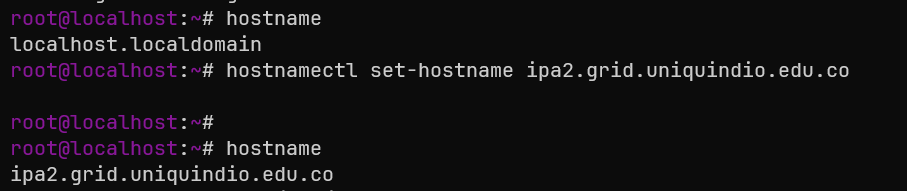
\includegraphics[width=0.8\textwidth]{mainmatter/II-desarrollo-metodologico/implementacion/imagenes/nombre-host-ipa2.png}
	\caption{Configuración del \acs{FQDN} del servidor de réplica}
	\label{fig:nombre-host-ipa2}
\end{figure}

Posteriormente, se habilitaron los servicios correspondientes a \ac{LDAP} y \ac{LDAPS} en el cortafuegos del sistema, con el fin de permitir la comunicación entre los diferentes componentes de la plataforma y garantizar el correcto funcionamiento de los servicios asociados a FreeIPA. En la \autoref{fig:reglas-cortafuegos-ipa2} se presenta la configuración aplicada.

\begin{figure}[H]
	\centering
	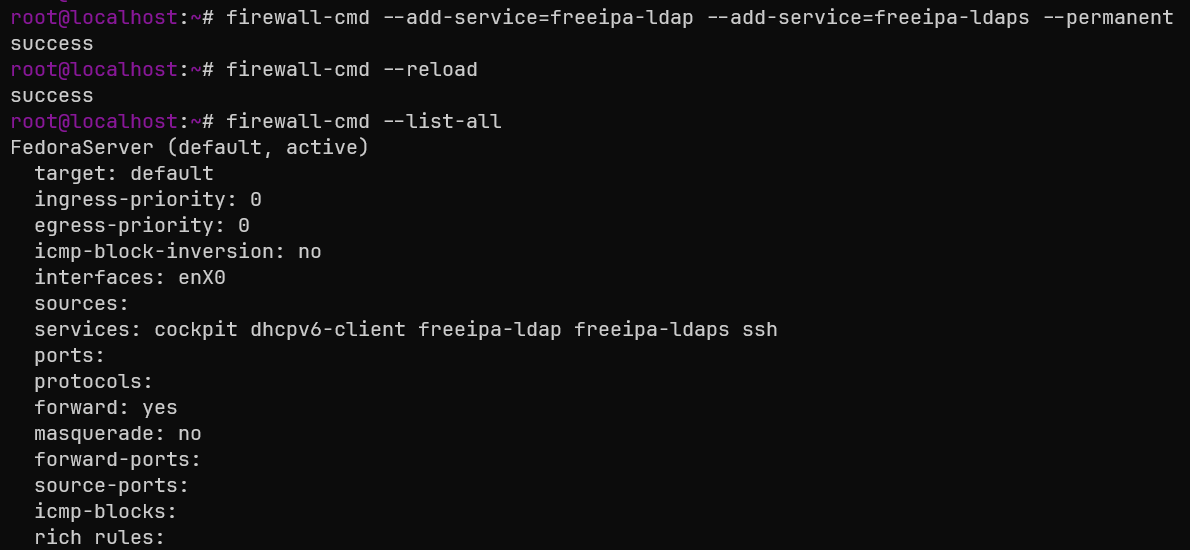
\includegraphics[width=0.8\textwidth]{mainmatter/II-desarrollo-metodologico/implementacion/imagenes/reglas-cortafuegos-ipa2.png}
	\caption{Configuración del cortafuegos del servidor de réplica}
	\label{fig:reglas-cortafuegos-ipa2}
\end{figure}

A continuación, se instaló el paquete freeipa-server, que incorpora las herramientas y dependencias necesarias para la implementación del servidor. En la \autoref{fig:instalacion-paquete-ipa2} se observa el procedimiento realizado.

\begin{figure}[H]
	\centering
	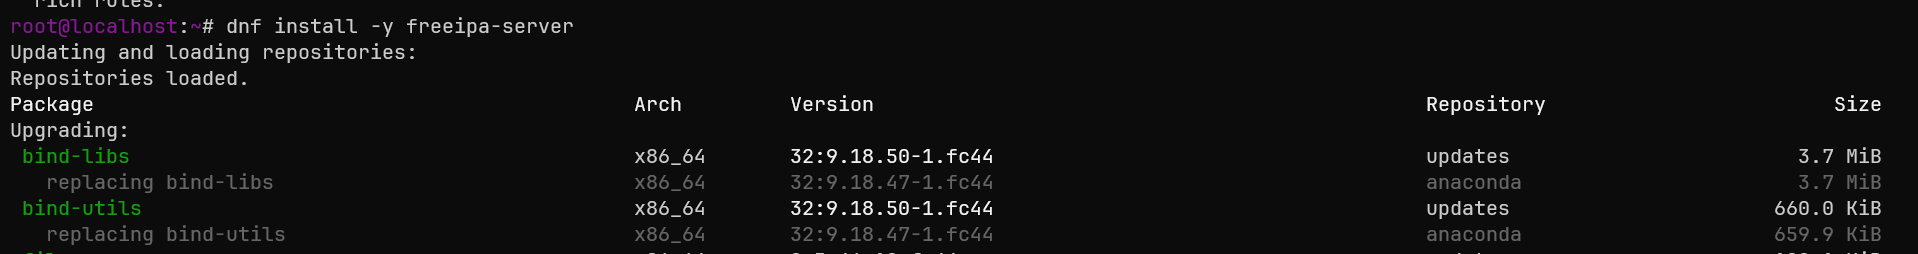
\includegraphics[width=0.8\textwidth]{mainmatter/II-desarrollo-metodologico/implementacion/imagenes/instalacion-paquete-ipa2.png}
	\caption{Instalación del paquete freeipa-server}
	\label{fig:instalacion-paquete-ipa2}
\end{figure}

Una vez completado este proceso, se instaló el cliente de FreeIPA, estableciendo la comunicación entre el servidor principal y el nuevo nodo de la infraestructura. El procedimiento de instalación correspondiente se presenta en la \autoref{fig:instalacion-cliente-ipa2}.

\begin{figure}[H]
	\centering
	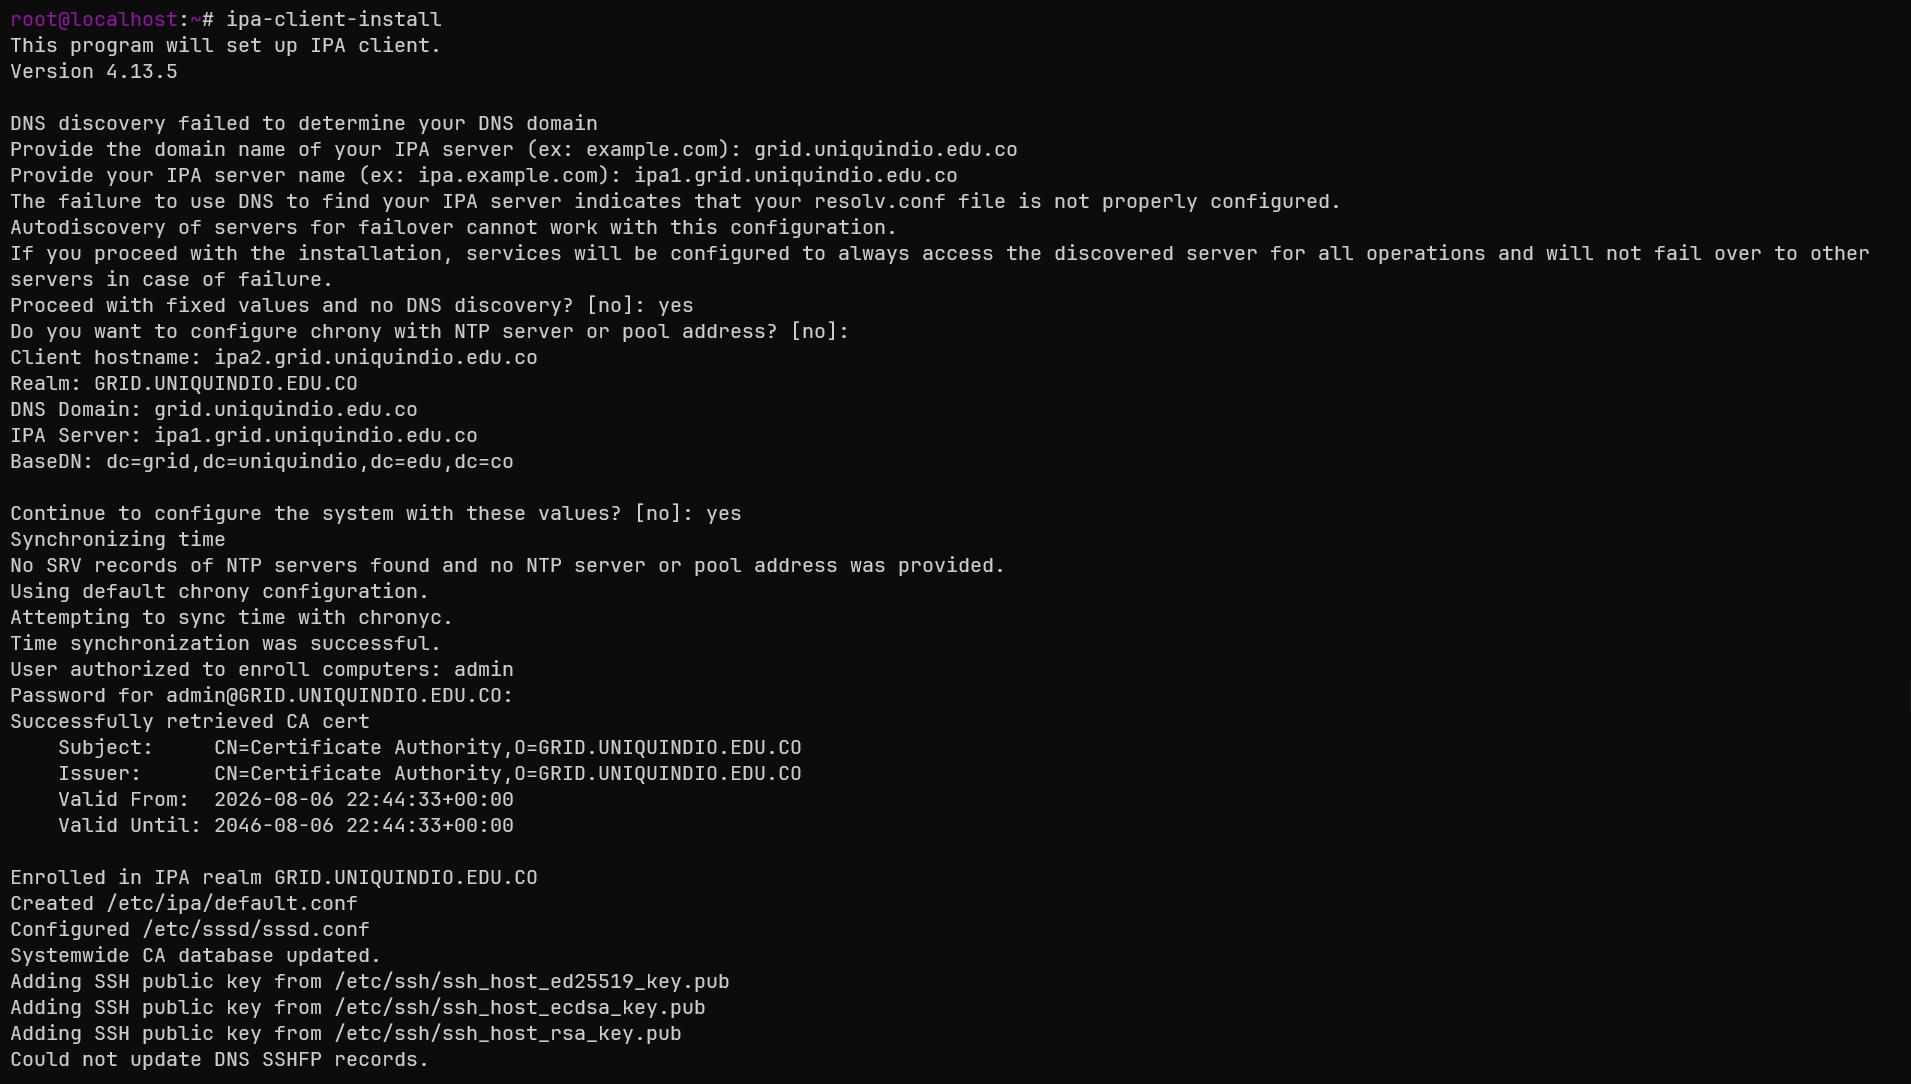
\includegraphics[width=0.8\textwidth]{mainmatter/II-desarrollo-metodologico/implementacion/imagenes/instalacion-cliente-ipa2.png}
	\caption{Instalación del cliente de FreeIPA}
	\label{fig:instalacion-cliente-ipa2}
\end{figure}

Posteriormente, desde el servidor principal se añadió el nuevo equipo al grupo ipaservers, lo que permitió conceder los permisos necesarios para que el sistema pudiera asumir el rol de servidor de réplica. Este procedimiento se muestra en la \autoref{fig:adicion-ipa2-a-ipa1}.

\begin{figure}[H]
	\centering
	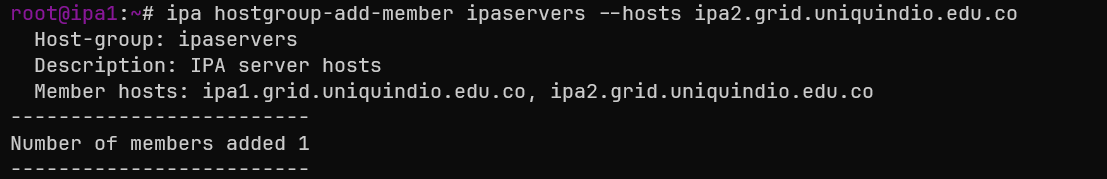
\includegraphics[width=0.8\textwidth]{mainmatter/II-desarrollo-metodologico/implementacion/imagenes/adicion-ipa2-a-ipa1.png}
	\caption{Incorporación del servidor al grupo ipaservers}
	\label{fig:adicion-ipa2-a-ipa1}
\end{figure}

Finalmente, se ejecutó el proceso de promoción del cliente a servidor de réplica, mediante el cual se llevó a cabo la instalación de los componentes necesarios y la sincronización de la información almacenada en el servidor principal. Una vez concluido el procedimiento, se verificó la incorporación del nuevo nodo a la infraestructura, comprobando que este apareciera en el listado de servidores registrados en la plataforma. El proceso de promoción se presenta en la \autoref{fig:promocion-cliente-servidor}, mientras que la \autoref{fig:verificacion-servidor-replica} muestra la verificación de la réplica creada.

\begin{figure}[H]
	\centering
	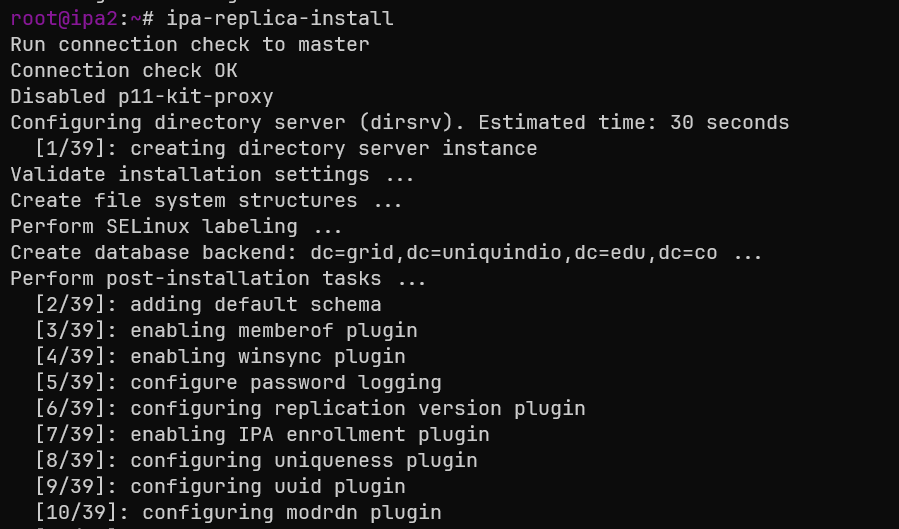
\includegraphics[width=0.8\textwidth]{mainmatter/II-desarrollo-metodologico/implementacion/imagenes/promocion-cliente-servidor.png}
	\caption{Promoción del cliente a servidor de réplica}
	\label{fig:promocion-cliente-servidor}
\end{figure}

\begin{figure}[H]
	\centering
	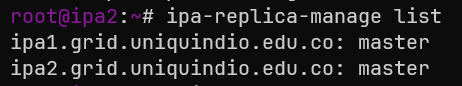
\includegraphics[width=0.8\textwidth]{mainmatter/II-desarrollo-metodologico/implementacion/imagenes/verificacion-servidor-replica.png}
	\caption{Verificación del servidor de réplica}
	\label{fig:verificacion-servidor-replica}
\end{figure}

\section{Instalación de HAProxy}\label{sec:instalacion-haproxy}

Con el fin de proporcionar redundancia y favorecer la disponibilidad y continuidad del servicio de directorio, la arquitectura propuesta contempla el despliegue de dos servidores FreeIPA. Esta decisión se tomó debido a que algunos de los servicios integrados con el directorio no disponen de mecanismos nativos de failover, por lo que no es posible definir automáticamente un servidor alternativo cuando uno de los servidores deja de estar disponible.

En este contexto, HAProxy proporciona un único punto de acceso al servicio de directorio y distribuye las solicitudes entre el servidor principal y el servidor de réplica mediante el algoritmo Round Robin. De esta forma, mientras ambos servidores se encuentren disponibles, las solicitudes son distribuidas entre ellos. Adicionalmente, se configuraron comprobaciones de disponibilidad (health checks) mediante \ac{LDAP}, permitiendo que HAProxy identifique cuándo un servidor deja de responder y lo retire temporalmente del conjunto de servidores disponibles. Así, las solicitudes continúan siendo atendidas por el servidor que permanece operativo, contribuyendo a garantizar la continuidad de los procesos de autenticación y autorización.

Como primer paso, se creó la máquina virtual destinada a alojar HAProxy. Para ello, se utilizó una plantilla basada en Debian 12 (Bookworm), asignando un procesador virtual, 1 \ac{GB} de memoria \acs{RAM} y 10 \ac{GB} de almacenamiento. Estos recursos fueron definidos de acuerdo con las características del servicio, considerando que HAProxy actúa como un componente ligero encargado principalmente de recibir, verificar y redirigir las conexiones hacia los servidores FreeIPA. La configuración utilizada para la creación de la máquina virtual se muestra en la \autoref{fig:configuracion-vm-haproxy}.

\begin{figure}[H]
	\centering
	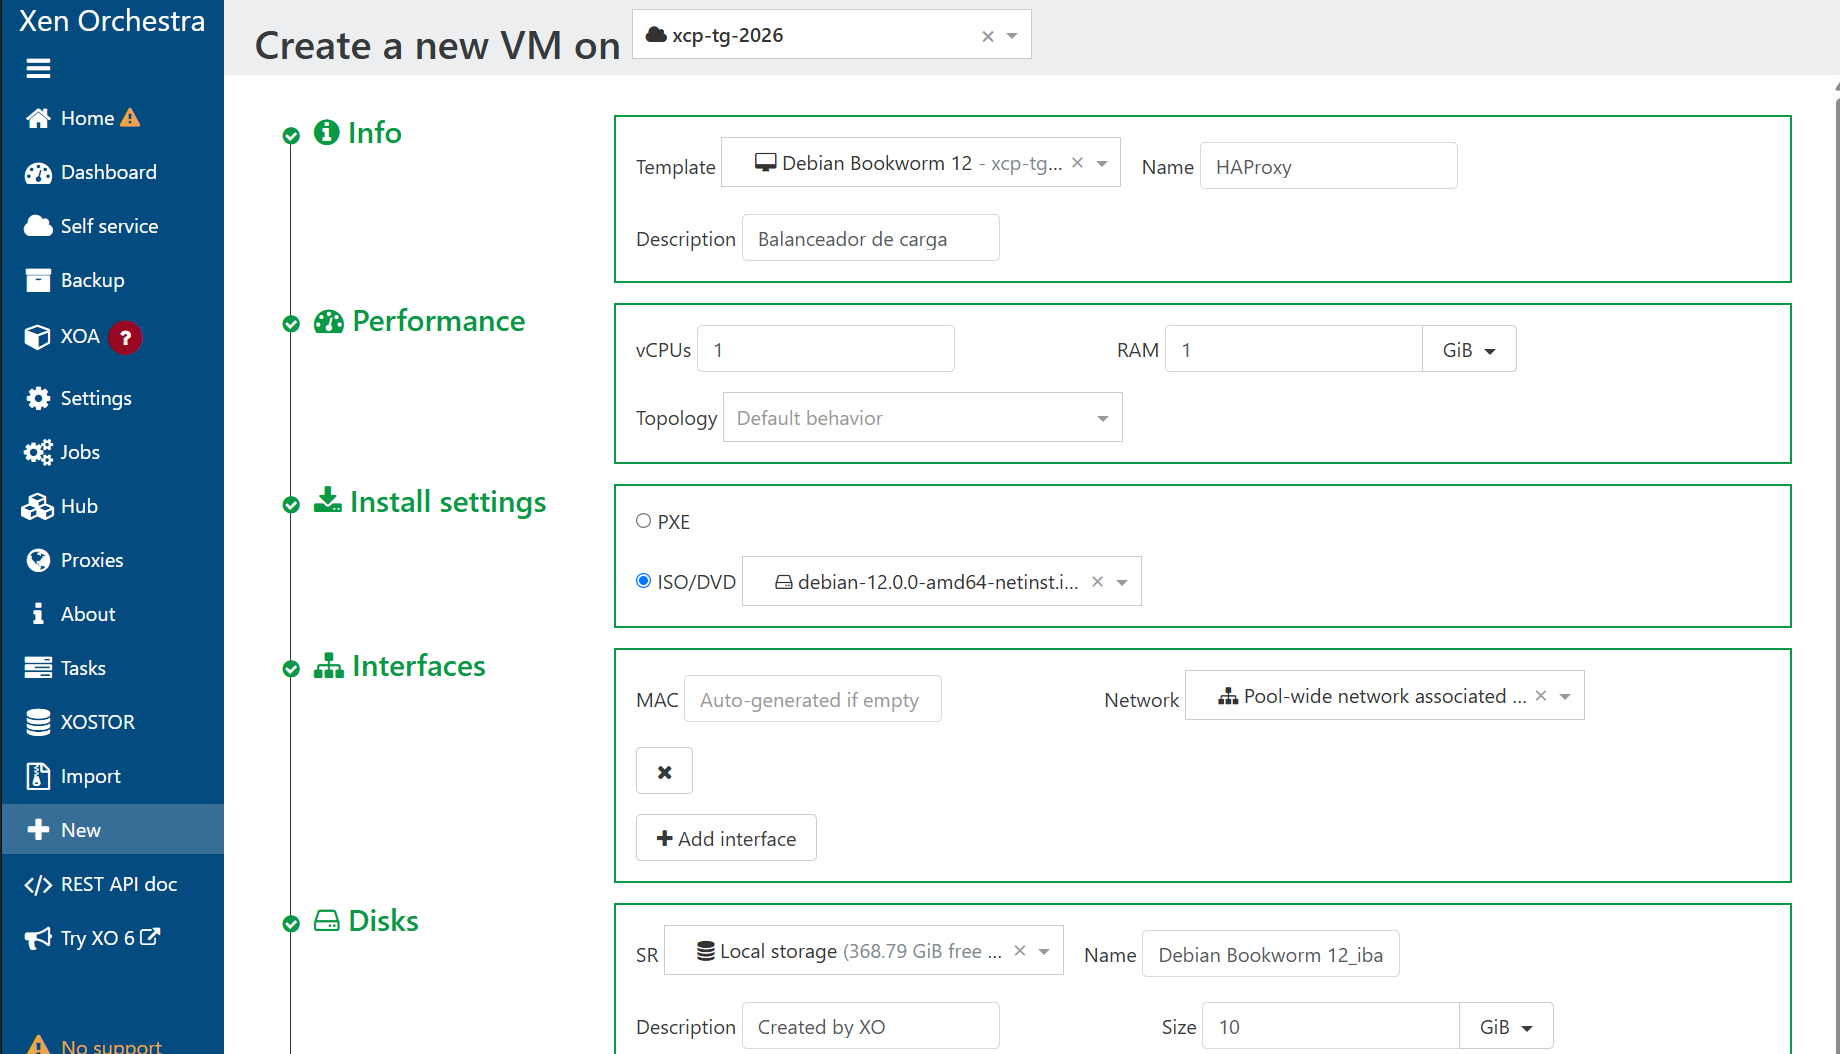
\includegraphics[width=0.8\textwidth]{mainmatter/II-desarrollo-metodologico/implementacion/imagenes/configuracion-vm-haproxy.png}
	\caption{Configuración de la máquina virtual destinada a la implementación de HAProxy}
	\label{fig:configuracion-vm-haproxy}
\end{figure}

Posteriormente, se realizó la instalación del sistema operativo y la configuración de la interfaz de red, asignando la dirección \acs{IP} 172.30.30.66 al servidor. Esta dirección permite identificar el balanceador dentro de la infraestructura y establecer la comunicación con los servidores FreeIPA. La configuración realizada se presenta en la \autoref{fig:configuracion-ip-haproxy}.

\begin{figure}[H]
	\centering
	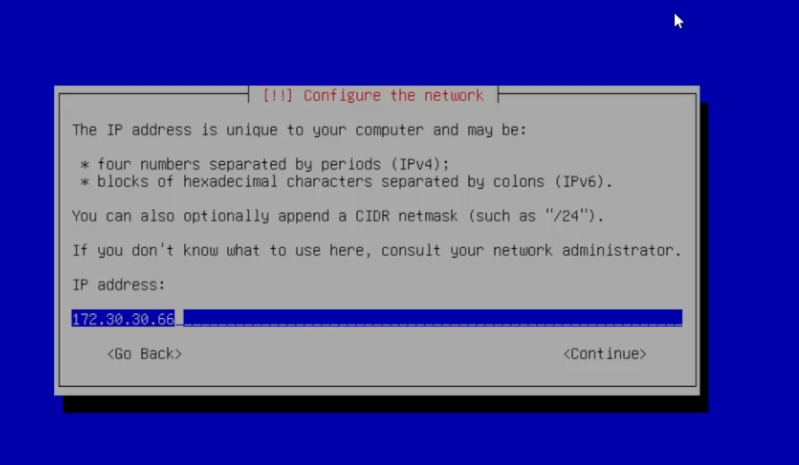
\includegraphics[width=0.8\textwidth]{mainmatter/II-desarrollo-metodologico/implementacion/imagenes/configuracion-ip-haproxy.png}
	\caption{Configuración de la dirección \acs{IP} del servidor HAProxy}
	\label{fig:configuracion-ip-haproxy}
\end{figure}

Una vez instalado y configurado el sistema operativo, se procedió con la instalación de HAProxy, estableciendo el componente encargado de recibir y gestionar las solicitudes dirigidas al servicio de directorio. En la \autoref{fig:instalacion-haproxy} se observa el proceso de instalación del balanceador.

\begin{figure}[H]
	\centering
	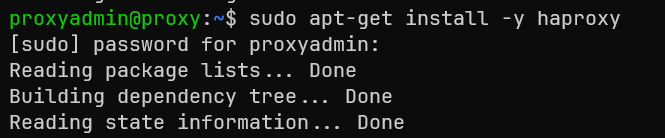
\includegraphics[width=0.8\textwidth]{mainmatter/II-desarrollo-metodologico/implementacion/imagenes/instalacion-haproxy.png}
	\caption{Instalación de HAProxy}
	\label{fig:instalacion-haproxy}
\end{figure}
Posteriormente, se configuró el archivo \texttt{/etc/haproxy/haproxy.cfg}, estableciendo los parámetros necesarios para que HAProxy pueda recibir y distribuir las conexiones del servicio de directorio tanto en su canal estándar como en su variante cifrada.

En primer lugar, para el tráfico \ac{LDAP} sin cifrado explícito, se definió el frontend \texttt{ft\_ldap}, encargado de recibir las conexiones en el puerto 389 mediante el modo \texttt{tcp} y con la opción \texttt{option tcplog} activada para el registro de tráficos. Este frontend transfiere las peticiones al backend \texttt{bk\_ldap}, donde se configuró el algoritmo \texttt{roundrobin} para distribuir la carga entre los servidores \texttt{ipa1} e \texttt{ipa2} (\texttt{ipa1.grid.uniquindio.edu.co} e \texttt{ipa2.grid.uniquindio.edu.co}). Asimismo, se incluyó la directiva \texttt{option ldap-check}, la cual realiza comprobaciones de salud específicas del protocolo \ac{LDAP} para determinar la disponibilidad de cada servidor antes de asignarle tráfico.

De forma complementaria, se estructuró la entrada para la comunicación cifrada \ac{LDAPS} mediante el frontend \texttt{ft\_ldaps}, configurado para recibir solicitudes en el puerto 636 bajo el modo \texttt{tcp}. Este remite las conexiones al backend \texttt{bk\_ldaps}, el cual balancea las peticiones cifradas entre los nodos \texttt{ipa1} e \texttt{ipa2} en el puerto 636 usando el algoritmo \texttt{roundrobin}. En este bloque, la validación de estado de los nodos se lleva a cabo mediante \texttt{option ssl-hello-chk}, asegurando que los servidores respondan adecuadamente al saludo inicial \ac{SSL}/\ac{TLS} antes de ser considerados operativos en el clúster. La configuración del frontend y backend utilizados para el balanceo se presenta en la \autoref{fig:configuracion-balanceo-freeipa-haproxy}.

\begin{figure}[H]
	\centering
	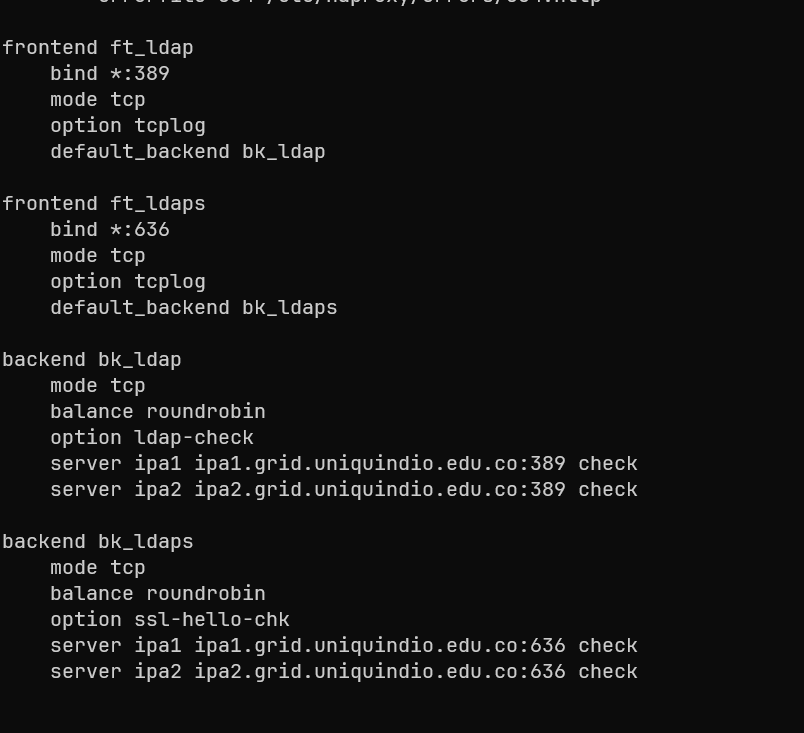
\includegraphics[width=0.8\textwidth]{mainmatter/II-desarrollo-metodologico/implementacion/imagenes/configuracion-balanceo-freeipa-haproxy.png}
	\caption{Configuración de HAProxy para el balanceo de los servidores FreeIPA}
	\label{fig:configuracion-balanceo-freeipa-haproxy}
\end{figure}

\subsection{Configuración del servicio \texorpdfstring{\acs{LDAP}}{LDAP} para el nombre virtual}

Para completar la integración entre HAProxy y FreeIPA, fue necesario registrar en FreeIPA el nombre \texttt{ipa.grid.uniquindio.edu.co} como un host. Este nombre representa el punto de acceso utilizado para el servicio de directorio a través del balanceador, diferenciándolo de los nombres individuales de los servidores \texttt{ipa1} e \texttt{ipa2}.

Para ello, se creó en FreeIPA un host fantasma (\textit{ghost host}) asociado al nombre \texttt{ipa.grid.uniquindio.edu.co}, utilizado para representar el nombre virtual mediante el cual se accederá al servicio de directorio a través de HAProxy. Para su creación se empleó el comando \texttt{ipa host-add} junto con los parámetros \texttt{-{}-random} y \texttt{-{}-force}. El parámetro \texttt{-{}-random} permite generar automáticamente una contraseña aleatoria para el host, mientras que \texttt{-{}-force} permite completar la creación del host fantasma bajo las condiciones requeridas por este procedimiento. Esta configuración permite registrar en FreeIPA el nombre virtual antes de asociarlo posteriormente con el servicio \ac{LDAP} utilizado por los servidores de la infraestructura. La creación del host fantasma se presenta en la \autoref{fig:creacion-host-servicio}.

\begin{figure}[H]
	\centering
	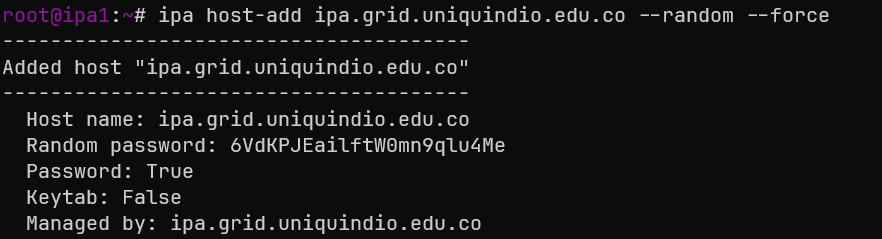
\includegraphics[width=0.8\textwidth]{mainmatter/II-desarrollo-metodologico/implementacion/imagenes/creacion-host-servicio.png}
	\caption{Creación del host destinado a la configuración del servicio}
	\label{fig:creacion-host-servicio}
\end{figure}

Una vez creado el host, se registró el servicio \ac{LDAP} asociado al nombre \nolinkurl{ipa.grid.uniquindio.edu.co} mediante el comando \texttt{ipa service-add}. Esta operación permite crear en FreeIPA el principal de servicio \nolinkurl{ldap/ipa.grid.uniquindio.edu.co@GRID.UNIQUINDIO.EDU.CO}, el cual identifica el servicio \ac{LDAP} que se utilizará bajo la identidad virtual. Esta configuración es fundamental para que la infraestructura de Kerberos y los mecanismos de autenticación de FreeIPA reconozcan correctamente el servicio, independientemente del servidor físico que atienda la solicitud. El proceso de adición del servicio se ilustra en la \autoref{fig:adicion-servicio-host}.

\begin{figure}[H]
	\centering
	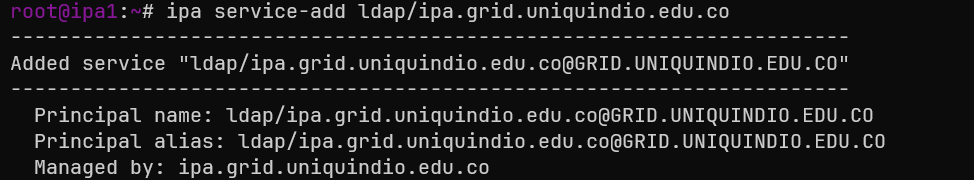
\includegraphics[width=0.8\textwidth]{mainmatter/II-desarrollo-metodologico/implementacion/imagenes/adicion-servicio-host.png}
	\caption{Adición del servicio al host configurado}
	\label{fig:adicion-servicio-host}
\end{figure}

Posteriormente, el servicio \ac{LDAP} se asoció tanto al servidor principal ipa1 como al servidor de réplica ipa2. De esta manera, ambos servidores quedan registrados como miembros del mismo servicio \ac{LDAP}, permitiendo que el nombre virtual utilizado por los clientes pueda ser atendido por cualquiera de los dos nodos de FreeIPA. Esta configuración constituye un mecanismo de redundancia para el acceso al servicio de directorio, ya que vincula el servicio lógico \nolinkurl{ldap/ipa.grid.uniquindio.edu.co} con los dos servidores que se encuentran detrás de HAProxy. La incorporación del servicio en ambos servidores se observa en la \autoref{fig:incorporacion-servicio-freeipa}.

\begin{figure}[H]
	\centering
	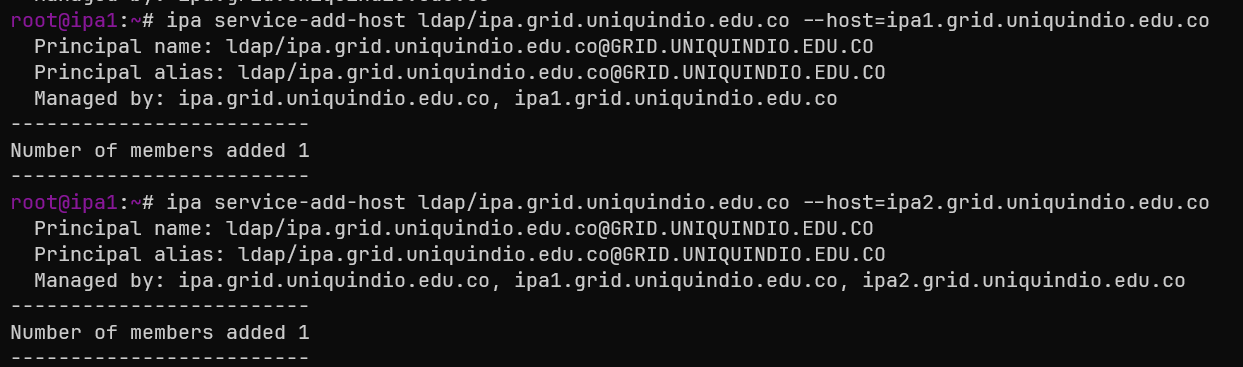
\includegraphics[width=0.8\textwidth]{mainmatter/II-desarrollo-metodologico/implementacion/imagenes/incorporacion-servicio-freeipa.png}
	\caption{Incorporación del servicio en los servidores FreeIPA}
	\label{fig:incorporacion-servicio-freeipa}
\end{figure}

Posteriormente, se verificó la configuración del servicio mediante la consulta de sus propiedades en FreeIPA. Esta comprobación permitió confirmar que el principal \ac{LDAP} había sido creado correctamente y que los servidores ipa1 e ipa2 se encontraban asociados al servicio. El resultado de esta verificación se presenta en la \autoref{fig:verificacion-servicio-ldap-virtual}.

\begin{figure}[H]
	\centering
	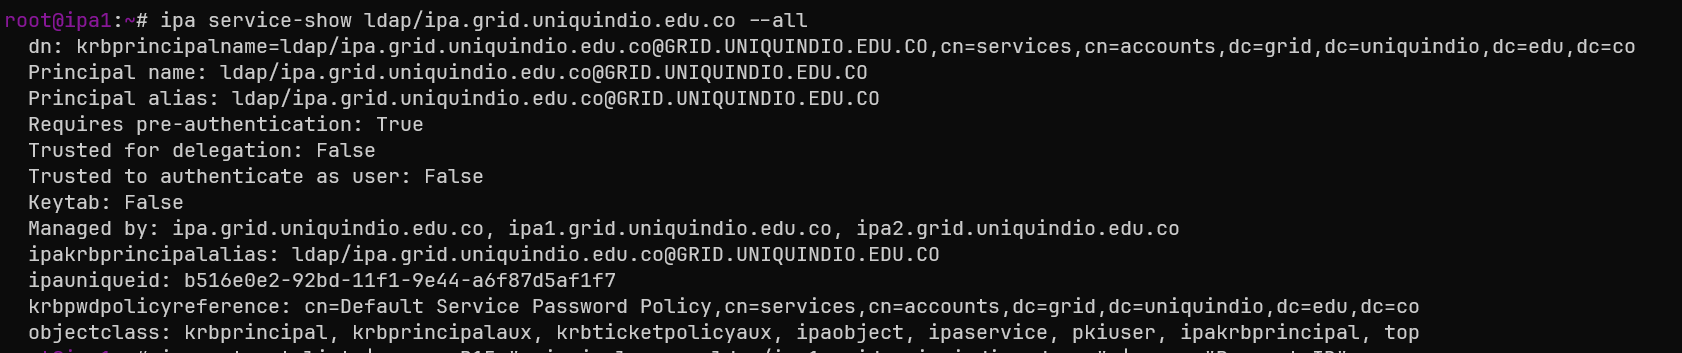
\includegraphics[width=0.8\textwidth]{mainmatter/II-desarrollo-metodologico/implementacion/imagenes/verificacion-servicio-ldap-virtual.png}
	\caption{Verificación del servicio \acs{LDAP} configurado para el nombre virtual}
	\label{fig:verificacion-servicio-ldap-virtual}
\end{figure}

\subsection{Configuración y validación de certificados}

Como parte de la configuración del acceso al servicio mediante el nombre virtual, se procedió a verificar y gestionar los certificados asociados a los servidores FreeIPA. Este procedimiento es necesario porque las conexiones \ac{LDAP} protegidas mediante \ac{TLS} utilizan el certificado digital del servidor para validar su identidad y, por tanto, el nombre utilizado para establecer la conexión debe estar contemplado en el certificado.

En el servidor principal se consultó la solicitud de certificado correspondiente al servicio y posteriormente se realizó su actualización mediante ipa-getcert. En este proceso se incluyó ipa.grid.uniquindio.edu.co como nombre \ac{DNS} asociado al certificado, además del nombre propio del servidor. Esto permite que el certificado pueda ser validado cuando la conexión se realice utilizando el nombre virtual definido para el servicio. En la \autoref{fig:certificado-servicio-servidor-principal} se observa la solicitud y el estado de monitorización del certificado en ipa1.

\begin{figure}[H]
	\centering
	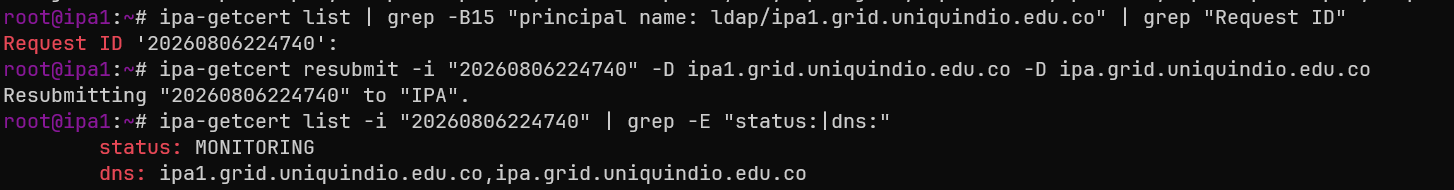
\includegraphics[width=0.8\textwidth]{mainmatter/II-desarrollo-metodologico/implementacion/imagenes/certificado-servicio-servidor-principal.png}
	\caption{Configuración y verificación del certificado del servicio en el servidor principal}
	\label{fig:certificado-servicio-servidor-principal}
\end{figure}

Finalmente, se realizó el mismo procedimiento en el servidor de réplica ipa2, verificando que el certificado asociado incluyera el nombre virtual utilizado para el servicio. La comprobación del estado MONITORING permite verificar que FreeIPA continúa gestionando la solicitud de certificado y que los nombres \ac{DNS} asociados al certificado corresponden a los nombres definidos para la infraestructura. La verificación realizada en el servidor de réplica se presenta en la \autoref{fig:certificado-servicio-servidor-replica}.

\begin{figure}[H]
	\centering
	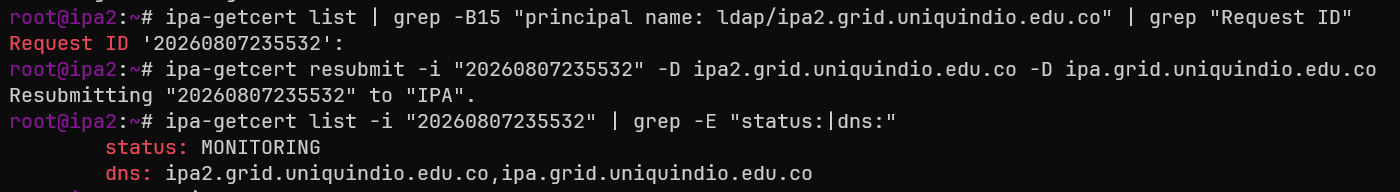
\includegraphics[width=0.8\textwidth]{mainmatter/II-desarrollo-metodologico/implementacion/imagenes/certificado-servicio-servidor-replica.png}
	\caption{Configuración y verificación del certificado del servicio en el servidor de réplica}
	\label{fig:certificado-servicio-servidor-replica}
\end{figure}

\section{Integración con los servicios}\label{sec:integracion-servicios}

Una vez configurado el balanceador, se realizó la conexión de los servicios con FreeIPA. Para ello, se utilizó la identidad asociada al balanceador de carga, representada mediante el nombre virtual ipa.grid.uniquindio.edu.co. Esta identidad permite que los servicios integrados utilicen un único punto de acceso al directorio, delegando en HAProxy la distribución de las solicitudes entre el servidor principal y la réplica, de acuerdo con su disponibilidad. De esta manera, los servicios no necesitan establecer una dependencia directa con un servidor específico de FreeIPA, sino que utilizan la identidad común definida para la solución.

\subsection{OpenVPN}\label{subsec:integracion-openvpn}

Para realizar la integración de OpenVPN con el servicio de gestión de identidades FreeIPA mediante el protocolo \ac{LDAP}, fue necesario instalar previamente el complemento openvpn-auth-ldap. Este componente permite que el servidor OpenVPN utilice un directorio \ac{LDAP} como fuente para la autenticación de los usuarios, delegando en FreeIPA la validación de las credenciales y la aplicación de las reglas de autorización definidas. Por esta razón, como primer paso se realizó la instalación del complemento mediante el gestor de paquetes del sistema operativo, como se observa en la \autoref{fig:instalacion-openvpn-autenticacion-ldap}.

\begin{figure}[H]
	\centering
	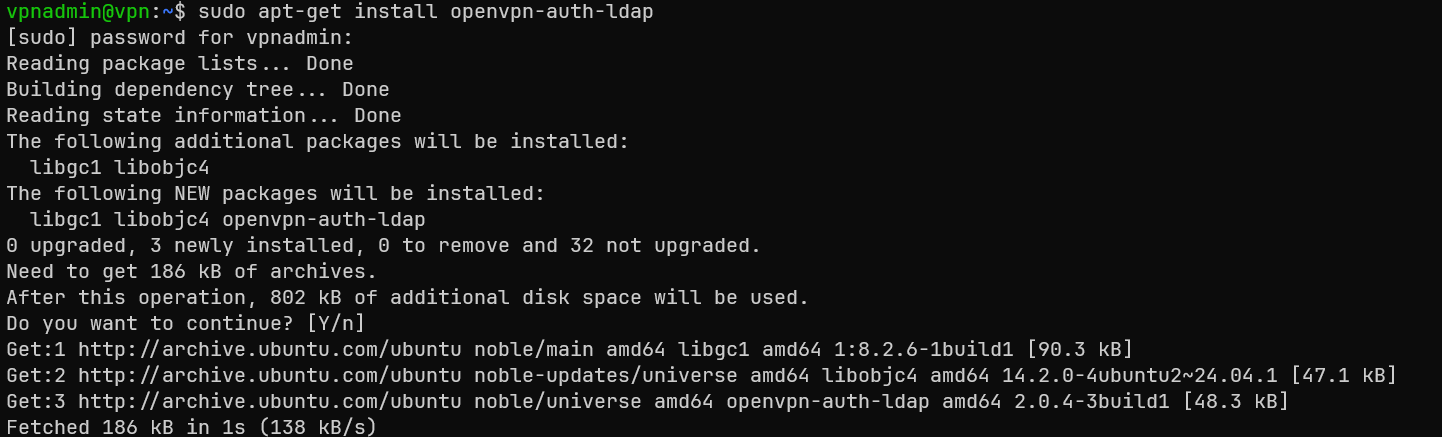
\includegraphics[width=0.8\textwidth]{mainmatter/II-desarrollo-metodologico/implementacion/imagenes/instalacion-openvpn-autenticacion-ldap.png}
	\caption{Instalación del complemento openvpn-auth-ldap}
	\label{fig:instalacion-openvpn-autenticacion-ldap}
\end{figure}

Para establecer la conexión \ac{LDAPS} entre OpenVPN y FreeIPA, primero fue necesario obtener el certificado de la autoridad certificadora (\acs{CA}) utilizada por FreeIPA. Desde la interfaz de línea de comandos del servidor FreeIPA, este certificado se encuentra disponible en la ruta /etc/ipa/ca.crt, desde donde puede ser copiado al servidor que ejecuta OpenVPN.

Como alternativa, el certificado puede obtenerse mediante la interfaz web de FreeIPA utilizando la URL \nolinkurl{https://ipa.grid.uniquindio.edu.co/ipa/config/ca.crt}. Al acceder a esta dirección se obtiene directamente el certificado de la autoridad certificadora utilizado por FreeIPA.

Una vez obtenido el certificado, se creó el archivo ca.crt en la ruta \path{/etc/openvpn/auth/ca.crt} del servidor OpenVPN, almacenando en este el certificado de la autoridad certificadora de FreeIPA. La disposición del certificado en esta ubicación permite utilizarlo como referencia para la validación de la conexión segura con el servicio \ac{LDAP} y constituye un elemento necesario para los siguientes pasos de configuración del complemento openvpn-auth-ldap. El archivo ca.crt en la ubicación correspondiente se muestra en la \autoref{fig:ubicacion-certificado-ca-openvpn}.

\begin{figure}[H]
	\centering
	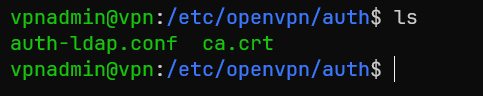
\includegraphics[width=0.8\textwidth]{mainmatter/II-desarrollo-metodologico/implementacion/imagenes/ubicacion-certificado-ca-openvpn.png}
	\caption{Archivo ca.crt ubicado en /etc/openvpn/auth/}
	\label{fig:ubicacion-certificado-ca-openvpn}
\end{figure}

Una vez instalado el complemento y ubicado el certificado de la autoridad certificadora en la ruta correspondiente, se procedió a configurar los parámetros necesarios para establecer la comunicación entre OpenVPN y FreeIPA. Esta configuración se realiza mediante el archivo auth-ldap.conf, utilizado por openvpn-auth-ldap para definir tanto los parámetros de conexión al directorio como los criterios mediante los cuales se buscan y autorizan los usuarios.

El paquete proporciona un archivo de configuración de ejemplo ubicado en \path{/usr/share/doc/openvpn-auth-ldap/examples/auth-ldap.conf}, el cual contiene diferentes parámetros para establecer una conexión \ac{LDAP}. A partir de este archivo se seleccionaron y adaptaron únicamente los parámetros necesarios para la infraestructura implementada. La configuración resultante se presenta en la \autoref{fig:configuracion-openvpn-autenticacion-ldap}.

\begin{figure}[H]
	\centering
	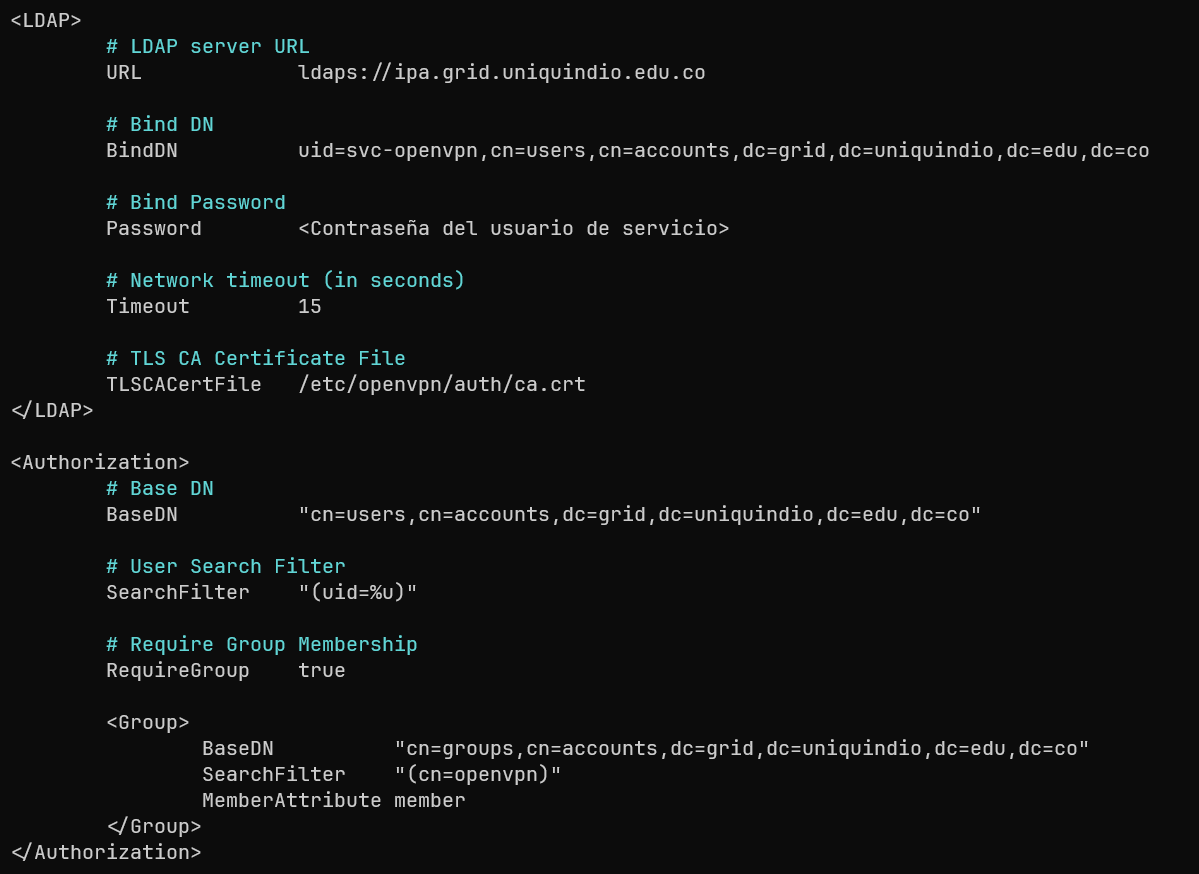
\includegraphics[width=0.8\textwidth]{mainmatter/II-desarrollo-metodologico/implementacion/imagenes/configuracion-openvpn-autenticacion-ldap.png}
	\caption{Configuración del complemento openvpn-auth-ldap para la integración con FreeIPA}
	\label{fig:configuracion-openvpn-autenticacion-ldap}
\end{figure}

Dentro del bloque \texttt{<LDAP>} se definieron inicialmente los parámetros relacionados con la conexión al servicio de directorio. El parámetro \texttt{URL} se configuró con el valor \nolinkurl{ldaps://ipa.grid.uniquindio.edu.co}, utilizando el nombre virtual asignado al servicio. De esta manera, OpenVPN no establece una dependencia directa con los nodos \texttt{ipa1} o \texttt{ipa2}, sino que dirige las solicitudes hacia HAProxy, el cual posteriormente determina cuál de los servidores FreeIPA disponibles atenderá la conexión.

Para realizar las consultas al directorio se configuró el parámetro \texttt{BindDN} con la cuenta de servicio \texttt{svc-openvpn}, utilizando su \ac{DN} completo:

\begin{center}
	\texttt{uid=svc-openvpn,cn=users,cn=accounts,dc=grid,dc=uniquindio,dc=co}
\end{center}

Esta cuenta se utiliza exclusivamente para que el servicio pueda realizar las consultas necesarias en FreeIPA y se encuentra separada de las cuentas personales de los usuarios. Su contraseña se establece mediante el parámetro \texttt{Password}. De esta manera, el complemento dispone de una identidad propia para realizar las operaciones de consulta contra el directorio.

También se estableció un tiempo máximo de espera de 15 segundos mediante el parámetro \texttt{Timeout}. Este valor determina cuánto tiempo esperará el complemento por una respuesta del servidor \ac{LDAP} antes de considerar que la comunicación no se ha completado correctamente.

A diferencia del archivo de ejemplo, en la configuración implementada no fue necesario habilitar explícitamente \texttt{TLSEnable}, debido a que la conexión se realiza directamente mediante \ac{LDAPS}, utilizando el esquema \texttt{ldaps://}. Para validar la identidad del servidor durante el establecimiento de la conexión segura, se especificó mediante \texttt{TLSCACertFile} el certificado de la autoridad certificadora de FreeIPA ubicado en \texttt{/etc/openvpn/auth/ca.crt}. Esto permite que OpenVPN pueda verificar que el certificado presentado por el servicio \ac{LDAP} es emitido por una autoridad de confianza.

En el bloque \texttt{<Authorization>} se definieron los parámetros encargados de determinar cómo se localizan y autorizan los usuarios dentro del directorio. El parámetro \texttt{BaseDN} se estableció en \texttt{cn=users,cn=accounts,dc=grid,dc=uniquindio,dc=co}, limitando las búsquedas de usuarios a la rama correspondiente a las cuentas de usuario de FreeIPA.

El parámetro \texttt{SearchFilter} se configuró como \texttt{(uid=\%u)}. El valor \texttt{\%u} es sustituido por el nombre de usuario proporcionado durante el inicio de sesión en OpenVPN. De esta manera, el complemento construye una búsqueda \ac{LDAP} que permite localizar dentro de FreeIPA la cuenta correspondiente al usuario que intenta autenticarse.

Además de validar que el usuario exista en el directorio, se estableció \texttt{RequireGroup true}, haciendo que la pertenencia a un grupo sea un requisito para completar la autorización. Esta configuración permite utilizar los grupos de FreeIPA como mecanismo de control de acceso al servicio OpenVPN, evitando que cualquier usuario registrado en el directorio pueda acceder automáticamente al servicio.

Para aplicar esta restricción se configuró el bloque \texttt{<Group>}. En este se estableció como \texttt{BaseDN} la rama \texttt{cn=groups,cn=accounts,dc=grid,dc=uniquindio,dc=co}, correspondiente a los grupos administrados por FreeIPA. El parámetro \texttt{SearchFilter} se configuró como \texttt{(cn=openvpn)}, por lo que el complemento busca específicamente el grupo \texttt{openvpn}.

Finalmente, se estableció \texttt{MemberAttribute member}, indicando el atributo utilizado por FreeIPA para determinar la pertenencia de los usuarios al grupo. En consecuencia, para que un usuario pueda autenticarse mediante OpenVPN no es suficiente con que sus credenciales sean válidas: también debe pertenecer al grupo \texttt{openvpn} definido previamente en FreeIPA.

De esta manera, la configuración implementada establece un flujo en el que Open\-VPN recibe las credenciales del usuario, \texttt{openvpn-auth-ldap} realiza las consultas contra FreeIPA mediante el nombre virtual \texttt{ipa.grid.uniquindio.edu.co}, HAProxy distribuye la conexión entre los servidores disponibles y FreeIPA valida tanto la existencia del usuario como su pertenencia al grupo autorizado para utilizar el servicio. Esto permite integrar la autenticación y autorización de OpenVPN con la gestión centralizada de identidades implementada en la infraestructura.

Una vez finalizada la configuración del archivo \texttt{auth-ldap.conf}, se procedió a habilitar el complemento en el servidor OpenVPN. Para ello, fue necesario modificar el archivo de configuración del servidor, ubicado en \path{/etc/openvpn/server/server.conf}, agregando la directiva \texttt{plugin}. Esta permite indicar a OpenVPN qué complemento debe cargar y especificar el archivo de configuración que contiene los parámetros necesarios para la conexión con FreeIPA. La línea agregada fue la siguiente:

\begin{center}
	\texttt{plugin /usr/lib/openvpn/openvpn-auth-ldap.so /etc/openvpn/auth/auth-ldap.conf}
\end{center}

En la \autoref{fig:activacion-openvpn-autenticacion-ldap} se observa la incorporación de esta directiva en el archivo de configuración del servidor OpenVPN.

\begin{figure}[H]
	\centering
	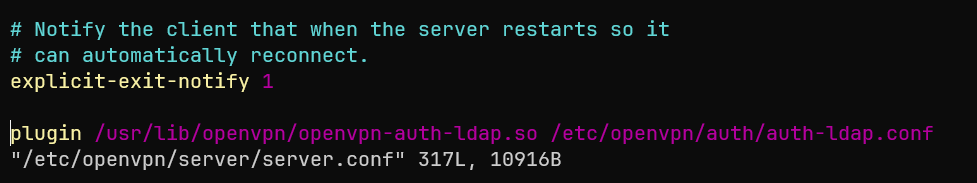
\includegraphics[width=0.8\textwidth]{mainmatter/II-desarrollo-metodologico/implementacion/imagenes/activacion-openvpn-autenticacion-ldap.png}
	\caption{Activación del complemento openvpn-auth-ldap en la configuración del servidor OpenVPN}
	\label{fig:activacion-openvpn-autenticacion-ldap}
\end{figure}

Finalmente, para que los clientes de OpenVPN puedan proporcionar las credenciales utilizadas para su autenticación mediante FreeIPA, fue necesario modificar el archivo de configuración .ovpn utilizado por el cliente. Para ello, se agregó la directiva auth-user-pass, la cual indica al cliente que debe solicitar las credenciales de usuario y contraseña durante el proceso de conexión. Esta configuración es necesaria para que las credenciales sean enviadas al servidor OpenVPN y puedan ser procesadas por el complemento openvpn-auth-ldap. En caso de no incluir esta directiva, el cliente no solicitará las credenciales requeridas y la autenticación mediante \ac{LDAP} no podrá completarse. La incorporación de la directiva auth-user-pass en el archivo de configuración del cliente se observa en la \autoref{fig:configuracion-autenticacion-cliente-openvpn}.

\begin{figure}[H]
	\centering
	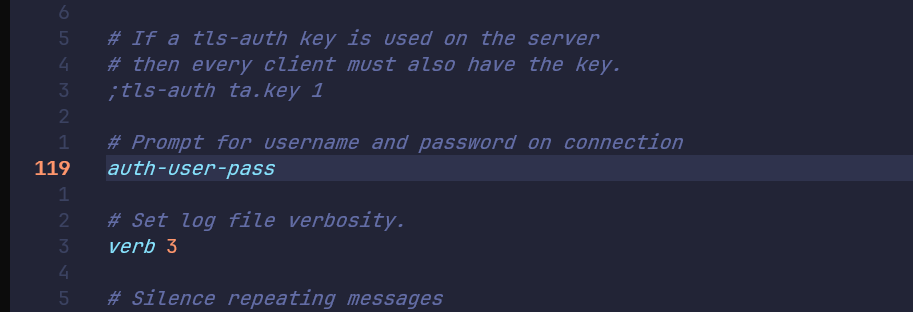
\includegraphics[width=0.8\textwidth]{mainmatter/II-desarrollo-metodologico/implementacion/imagenes/configuracion-autenticacion-cliente-openvpn.png}
	\caption{Configuración de autenticación mediante usuario y contraseña en el cliente OpenVPN}
	\label{fig:configuracion-autenticacion-cliente-openvpn}
\end{figure}

\subsection{OpenProject}\label{subsec:integracion-openproject}

Para realizar la integración de OpenProject con el servicio de directorio, fue necesario configurar una conexión \ac{LDAP} desde la interfaz de administración de la plataforma. Para acceder a esta configuración, se ingresó al menú Perfil → Administración → Autenticación → Conexiones \ac{LDAP}, desde donde es posible administrar las conexiones con servidores de directorio.

En esta sección se creó una nueva conexión \ac{LDAP}, en cuyo formulario se definieron inicialmente los parámetros básicos de comunicación con el servicio, incluyendo el nombre asignado a la conexión, el host o dirección del servicio \ac{LDAP} y el puerto utilizado para establecer la comunicación. En este caso, la conexión se configuró utilizando la identidad del servicio definida mediante \nolinkurl{ipa.grid.uniquindio.edu.co}, permitiendo que OpenProject utilice el punto de acceso proporcionado por HAProxy en lugar de establecer una conexión directa con un servidor específico de FreeIPA. Los parámetros iniciales de la conexión \ac{LDAP} configurada se presentan en la \autoref{fig:configuracion-inicial-ldap-openproject}.

\begin{figure}[H]
	\centering
	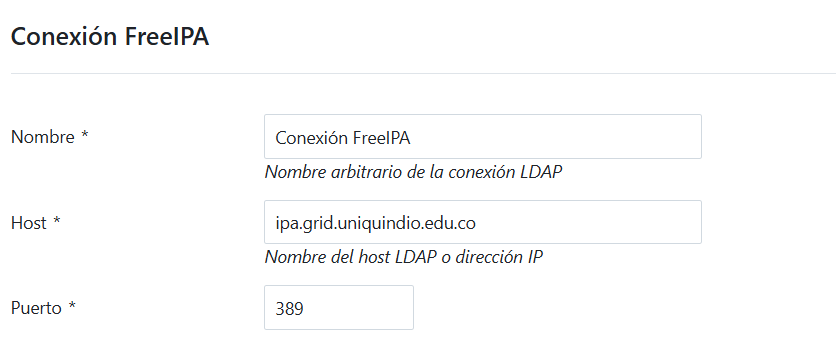
\includegraphics[width=0.8\textwidth]{mainmatter/II-desarrollo-metodologico/implementacion/imagenes/configuracion-inicial-ldap-openproject.png}
	\caption{Configuración inicial de la conexión \acs{LDAP} en OpenProject}
	\label{fig:configuracion-inicial-ldap-openproject}
\end{figure}

Posteriormente, se configuraron los parámetros relacionados con la seguridad de la conexión \ac{LDAP}. OpenProject permite seleccionar entre tres modalidades de conexión: sin cifrado, STARTTLS y \ac{LDAPS}. Debido a que el servicio de directorio se encuentra configurado para admitir tanto conexiones STARTTLS como \ac{LDAPS}, se seleccionó STARTTLS, opción recomendada por OpenProject para establecer una conexión \ac{LDAP} protegida mediante \ac{TLS}.

Adicionalmente, se habilitó la opción de validación del certificado \ac{SSL}, con el propósito de verificar la identidad del servidor durante el establecimiento de la conexión y mantener la seguridad de las comunicaciones. Al activar esta opción, OpenProject permite proporcionar el certificado de la autoridad certificadora utilizada para validar el certificado presentado por el servicio \ac{LDAP}. Para este caso, se incorporó el certificado de la \acs{CA} de FreeIPA previamente obtenido, permitiendo que OpenProject pueda validar la cadena de confianza al establecer la conexión mediante ipa.grid.uniquindio.edu.co. La configuración de seguridad \ac{TLS} y validación del certificado se muestra en la \autoref{fig:seguridad-tls-certificado-openproject}.

\begin{figure}[H]
	\centering
	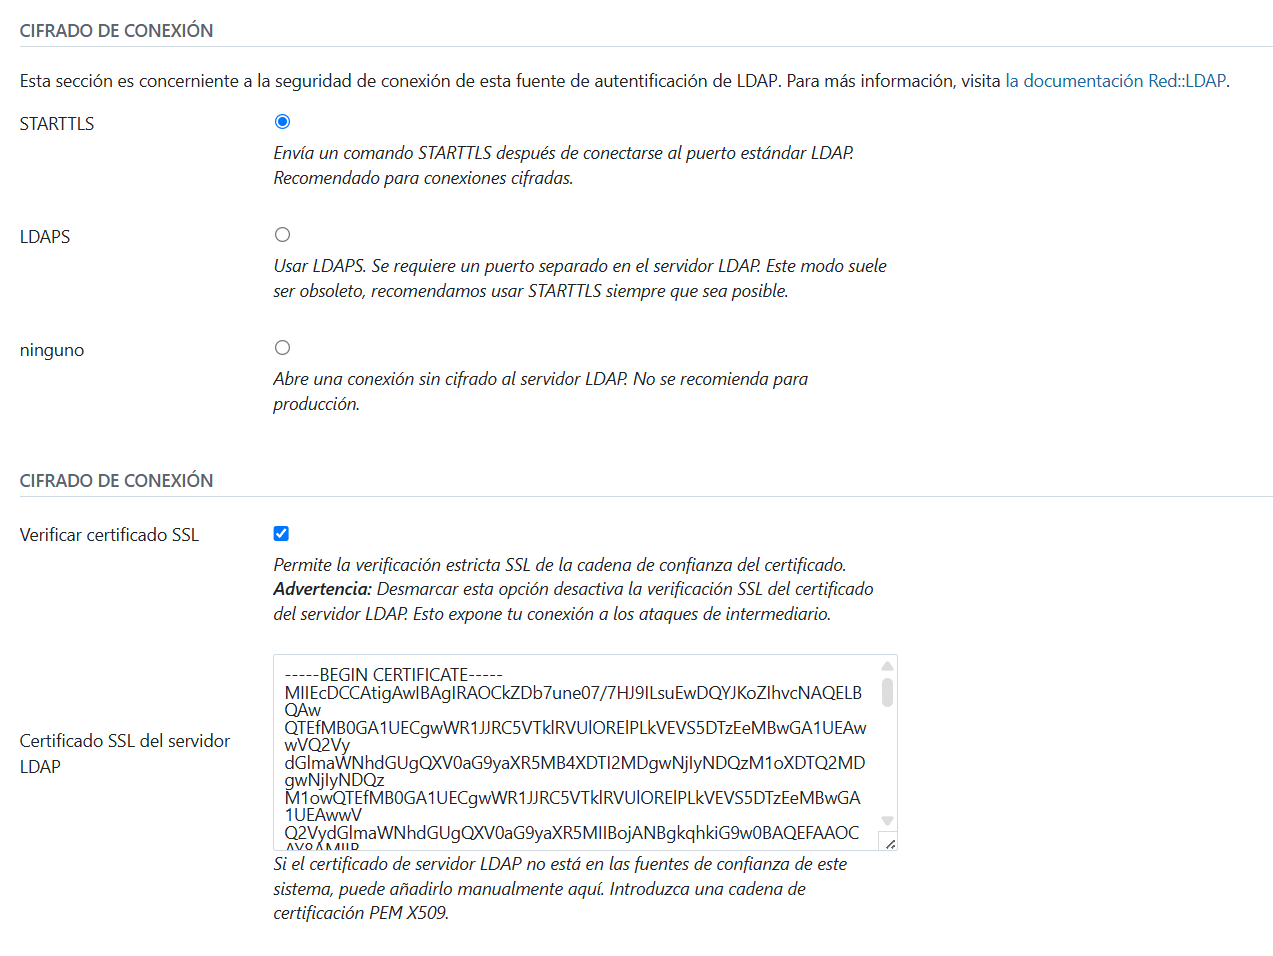
\includegraphics[width=0.8\textwidth]{mainmatter/II-desarrollo-metodologico/implementacion/imagenes/seguridad-tls-certificado-openproject.png}
	\caption{Configuración de seguridad \acs{TLS} y validación del certificado de la conexión \acs{LDAP}}
	\label{fig:seguridad-tls-certificado-openproject}
\end{figure}

El siguiente apartado corresponde a la configuración de la cuenta de servicio previamente creada para la integración con FreeIPA. Esta cuenta permite que OpenProject realice las consultas necesarias en el directorio \ac{LDAP} y, para ello, se deben proporcionar las credenciales con las que se establecerá dicha comunicación. En este formulario se definieron el \ac{DN} de la cuenta de servicio y su respectiva contraseña. El \ac{DN} utilizado fue \nolinkurl{uid=svc-openproject,cn=users,cn=accounts,dc=grid,dc=uniquindio,dc=co}, correspondiente a la cuenta de servicio creada específicamente para OpenProject. La configuración de la cuenta de servicio para la conexión \ac{LDAP} se presenta en la \autoref{fig:cuenta-servicio-ldap-openproject}.

\begin{figure}[H]
	\centering
	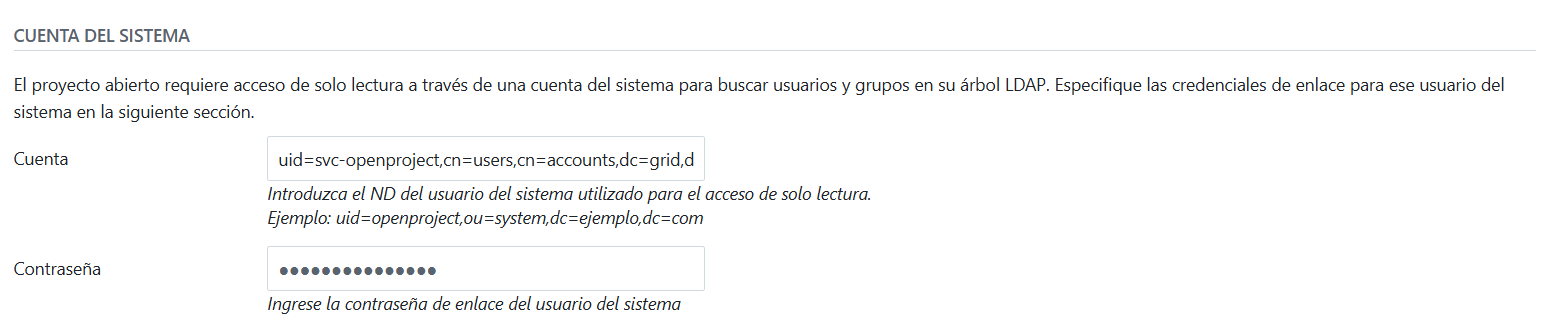
\includegraphics[width=0.8\textwidth]{mainmatter/II-desarrollo-metodologico/implementacion/imagenes/cuenta-servicio-ldap-openproject.png}
	\caption{Configuración de la cuenta de servicio para la conexión \acs{LDAP} de OpenProject}
	\label{fig:cuenta-servicio-ldap-openproject}
\end{figure}

Posteriormente, se configuraron los parámetros correspondientes a los detalles de búsqueda dentro del directorio \ac{LDAP}. En el campo \texttt{Base DN} se estableció \nolinkurl{dc=grid,dc=uniquindio,dc=edu,dc=co}, correspondiente a la raíz del directorio de FreeIPA. Esta configuración permite que OpenProject realice las búsquedas de usuarios y grupos dentro del dominio \ac{LDAP} definido para la infraestructura.

Para limitar los usuarios que pueden ser sincronizados y autenticarse mediante esta conexión, se definió el filtro \nolinkurl{(memberOf=cn=openproject,cn=groups,cn=accounts,dc=grid,dc=uniquindio,dc=edu,dc=co)} el cual está asociado al grupo openproject. De esta manera, OpenProject no considera de forma indiscriminada todas las cuentas existentes en FreeIPA, sino únicamente aquellas que cumplen con la pertenencia al grupo destinado al servicio. Esta configuración permite utilizar los grupos definidos previamente en FreeIPA como mecanismo de control de acceso para OpenProject.

Asimismo, se mantuvo habilitada la opción de creación automática de usuarios, permitiendo que una cuenta de FreeIPA que cumpla con los criterios establecidos pueda ser creada automáticamente en OpenProject durante su primera autenticación. Esto evita tener que crear manualmente en OpenProject cada una de las cuentas que ya se encuentran administradas desde el servicio centralizado de identidades. Los parámetros de búsqueda de usuarios configurados se observan en la \autoref{fig:base-dn-busqueda-openproject}.

\begin{figure}[H]
	\centering
	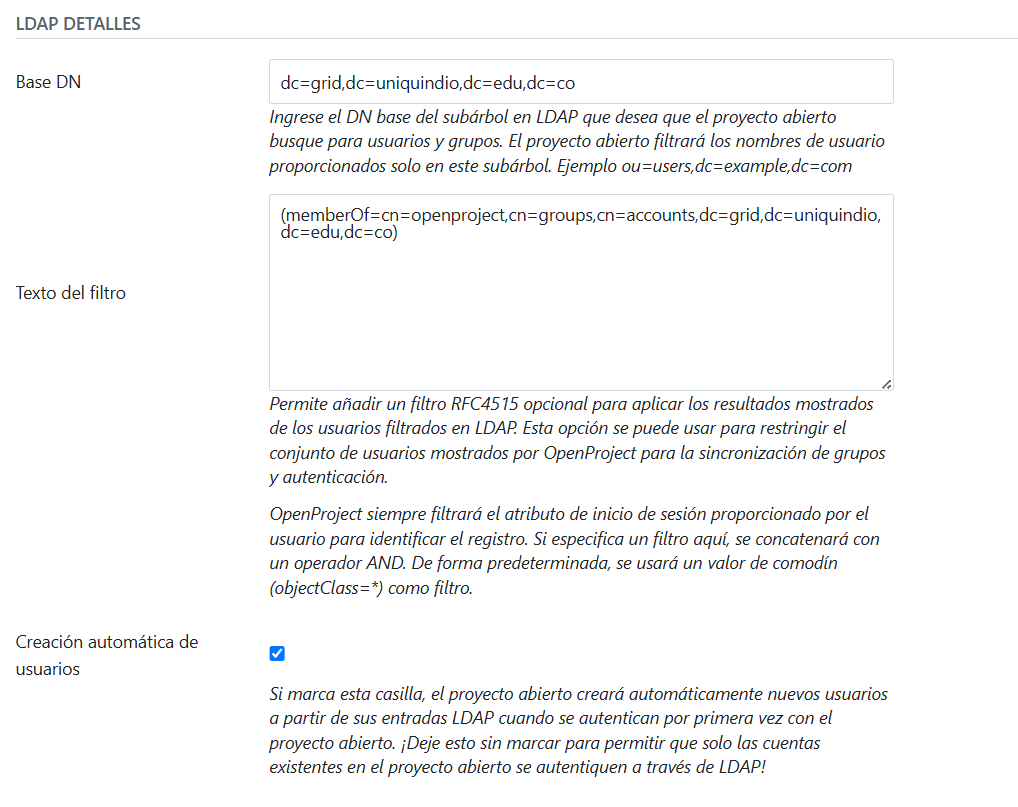
\includegraphics[width=0.8\textwidth]{mainmatter/II-desarrollo-metodologico/implementacion/imagenes/base-dn-busqueda-openproject.png}
	\caption{Configuración de la base \acs{DN} y los criterios de búsqueda de usuarios en OpenProject}
	\label{fig:base-dn-busqueda-openproject}
\end{figure}

Finalmente, se realizó el mapeo de atributos, mediante el cual se estableció la correspondencia entre los atributos definidos en las cuentas de usuario de FreeIPA y los campos utilizados por OpenProject. Esta configuración permite que, al crear o sincronizar un usuario a partir de una entrada \ac{LDAP}, OpenProject pueda identificar y asignar correctamente la información de la cuenta.

Para el nombre de usuario se definió el atributo uid, utilizado como identificador de inicio de sesión. Para el campo Nombre se estableció givenName, mientras que para Apellido se configuró sn. Finalmente, para el Correo electrónico se utilizó el atributo mail. Estos atributos corresponden a la información almacenada en las cuentas de usuario de FreeIPA y permiten que OpenProject complete los datos básicos del usuario a partir del directorio centralizado.

El campo Administrador se dejó sin configurar, debido a que no se utilizó un atributo \ac{LDAP} para determinar directamente los privilegios administrativos dentro de OpenProject. El mapeo de atributos configurado para la integración se presenta en la \autoref{fig:mapeo-atributos-ldap-openproject}.

\begin{figure}[H]
	\centering
	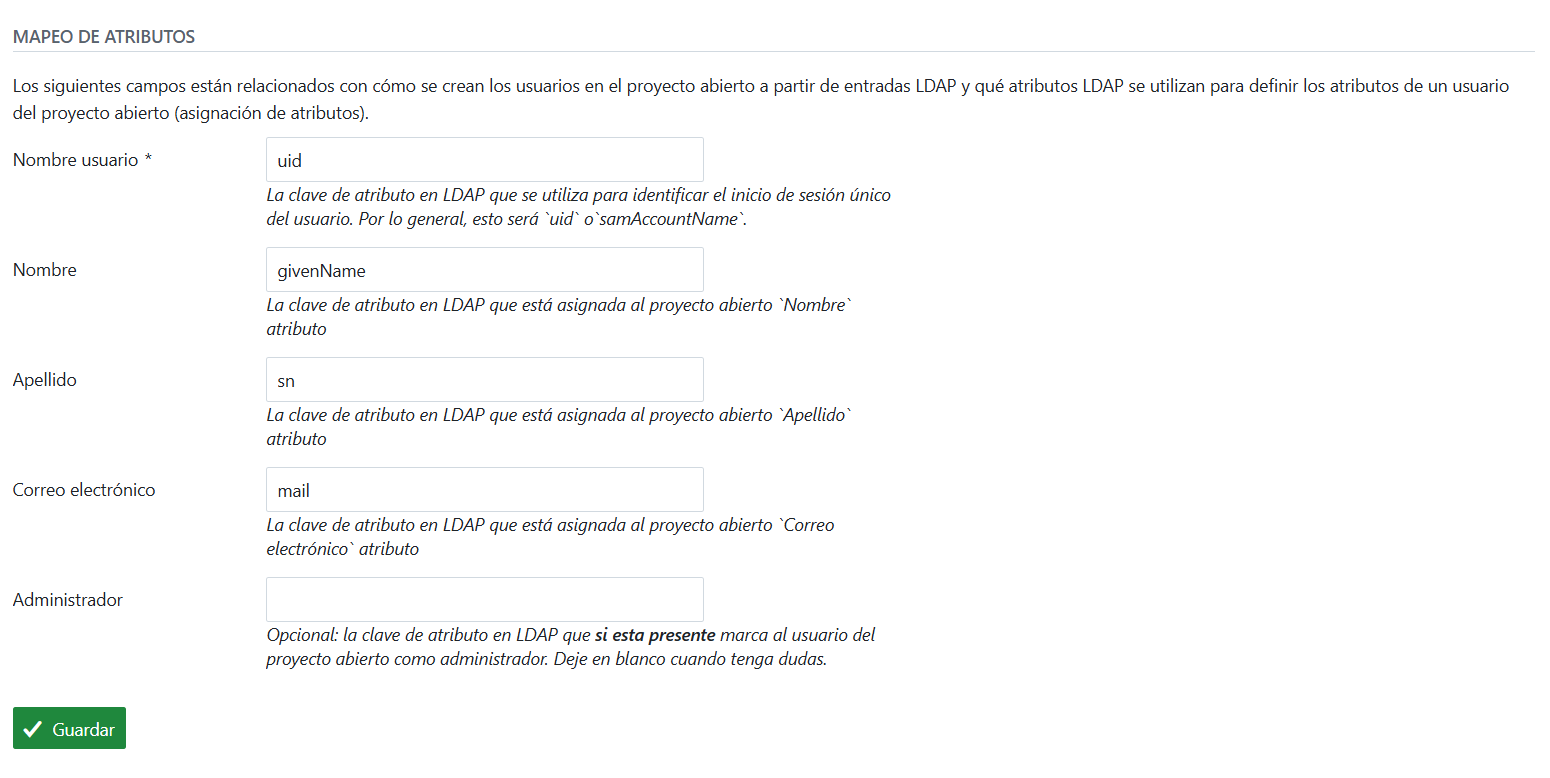
\includegraphics[width=0.8\textwidth]{mainmatter/II-desarrollo-metodologico/implementacion/imagenes/mapeo-atributos-ldap-openproject.png}
	\caption{Mapeo de atributos \acs{LDAP} para los usuarios de OpenProject}
	\label{fig:mapeo-atributos-ldap-openproject}
\end{figure}

Una vez guardada la configuración de la conexión \ac{LDAP}, OpenProject permite realizar una prueba para verificar la comunicación con el servicio de directorio y validar los parámetros configurados. Al ejecutar esta prueba, la plataforma confirmó que la conexión con el servicio FreeIPA se estableció correctamente, mostrando el mensaje «Conexión exitosa». Este resultado permite comprobar que los parámetros de conexión, seguridad y autenticación definidos previamente son aceptados por el servidor de directorio. La conexión \ac{LDAP} configurada y el resultado satisfactorio de la prueba de conectividad se muestran en la \autoref{fig:validacion-conexion-openproject-freeipa}.

\begin{figure}[H]
	\centering
	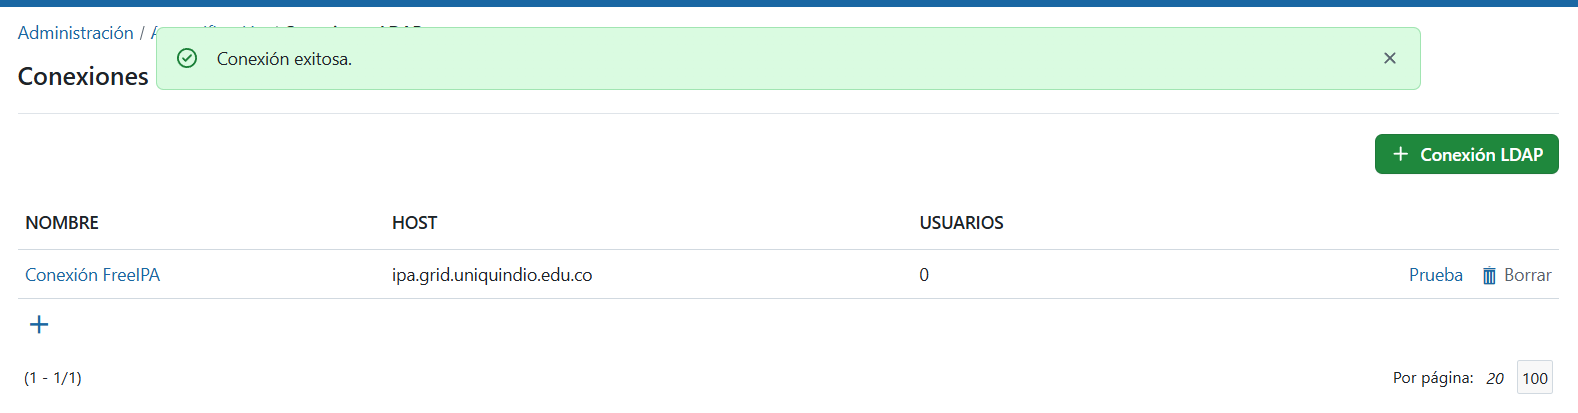
\includegraphics[width=0.8\textwidth]{mainmatter/II-desarrollo-metodologico/implementacion/imagenes/validacion-conexion-openproject-freeipa.png}
	\caption{Validación de la conexión entre OpenProject y FreeIPA}
	\label{fig:validacion-conexion-openproject-freeipa}
\end{figure}

\subsection{Xen Orchestra}\label{subsec:integracion-xen-orchestra}

Como primer paso, se procede a habilitar el complemento \ac{LDAP} en Xen Orchestra. Para ello, se ingresa a Configuración → Complementos (Plugins) y se localiza el complemento correspondiente a la autenticación \ac{LDAP}. Para habilitarlo, es necesario crear previamente una configuración asociada al complemento y guardarla. Una vez habilitado, se pueden establecer los diferentes parámetros requeridos para su integración con el servicio de directorio, los cuales son configurados en los siguientes pasos. El complemento \ac{LDAP} disponible en la sección de complementos se observa en la \autoref{fig:complemento-ldap-xen-orchestra}.

\begin{figure}[H]
	\centering
	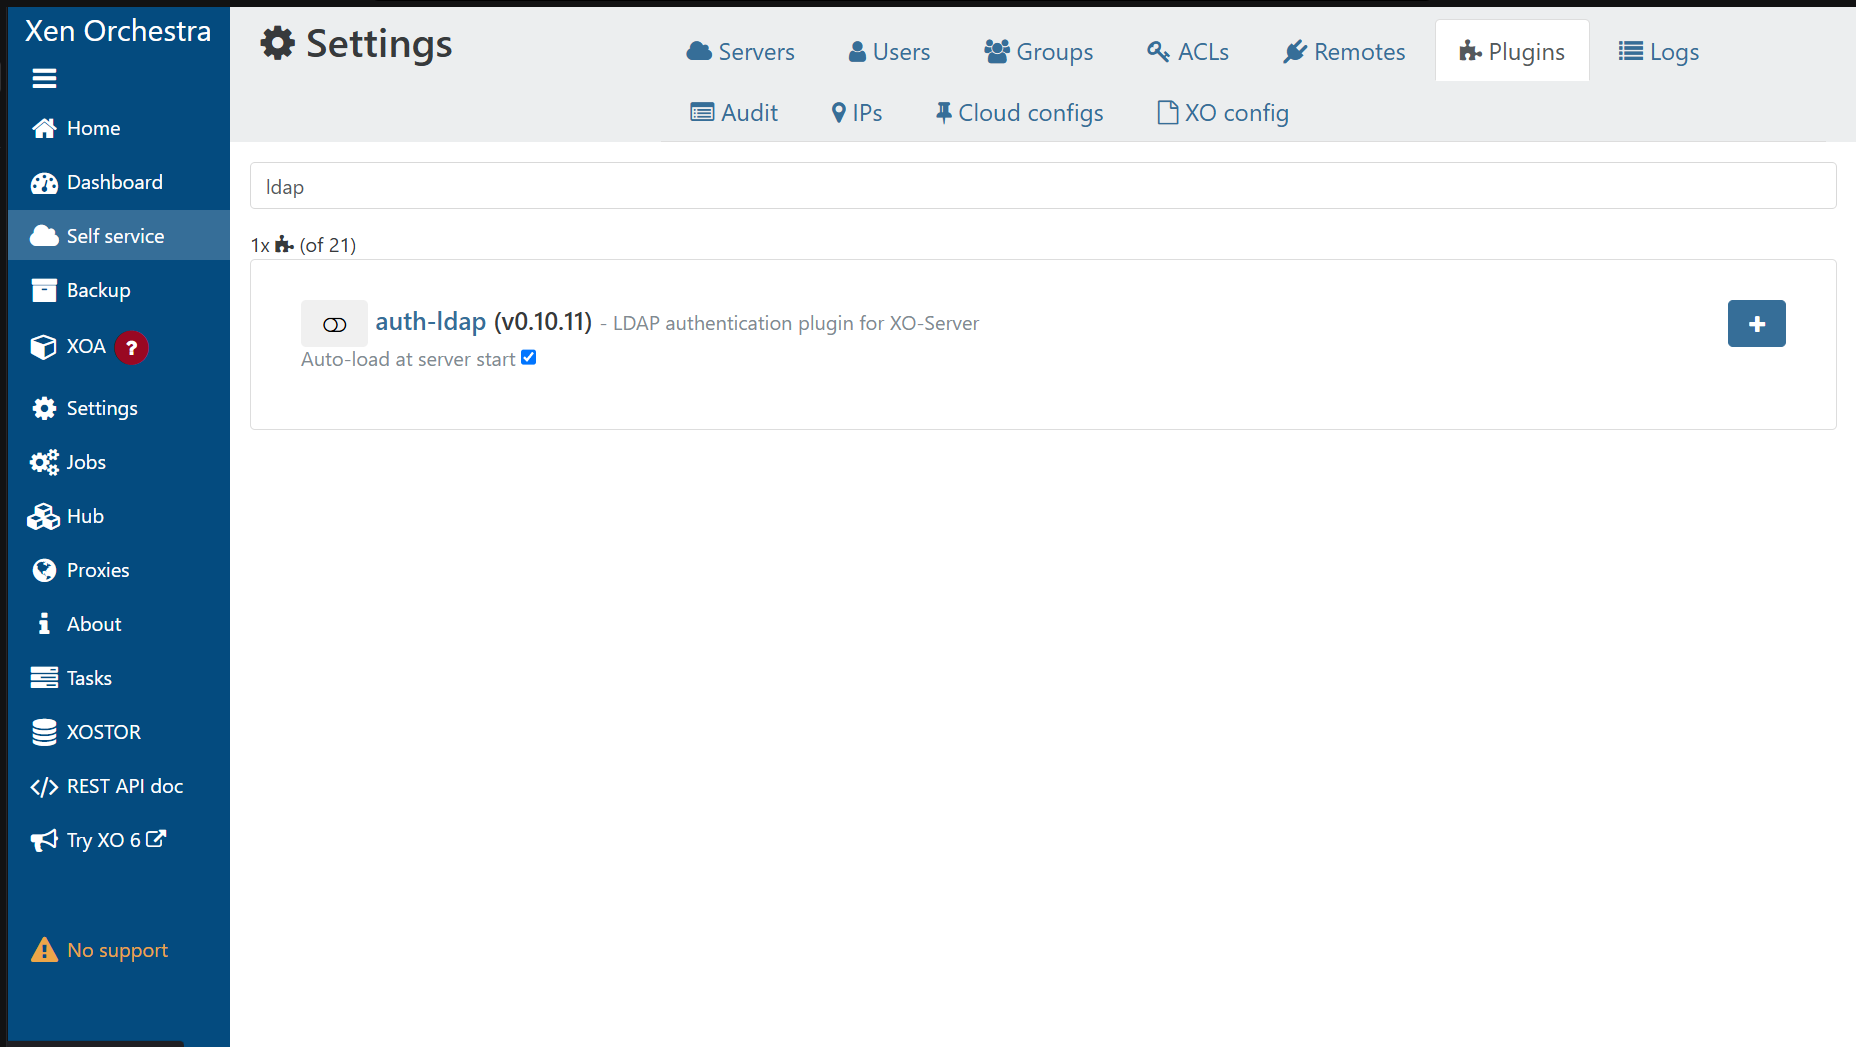
\includegraphics[width=0.8\textwidth]{mainmatter/II-desarrollo-metodologico/implementacion/imagenes/complemento-ldap-xen-orchestra.png}
	\caption{Complemento \acs{LDAP} disponible en Xen Orchestra}
	\label{fig:complemento-ldap-xen-orchestra}
\end{figure}

Para iniciar la configuración del complemento, el primer parámetro que se establece es la \ac{URI} del servidor \ac{LDAP}, la cual permite definir la dirección y el puerto mediante los que Xen Orchestra establece la comunicación con el servicio de directorio. En este caso, se utiliza la \ac{URI} \nolinkurl{ldap://ipa.grid.uniquindio.edu.co:389}, correspondiente al punto de acceso \ac{LDAP} definido para la infraestructura. Esta dirección permite que el complemento realice las consultas de autenticación contra el servicio de directorio a través de la identidad establecida para la infraestructura. La configuración de la \ac{URI} del servidor \ac{LDAP} en el complemento se muestra en la \autoref{fig:configuracion-uri-ldap-xen-orchestra}.

\begin{figure}[H]
	\centering
	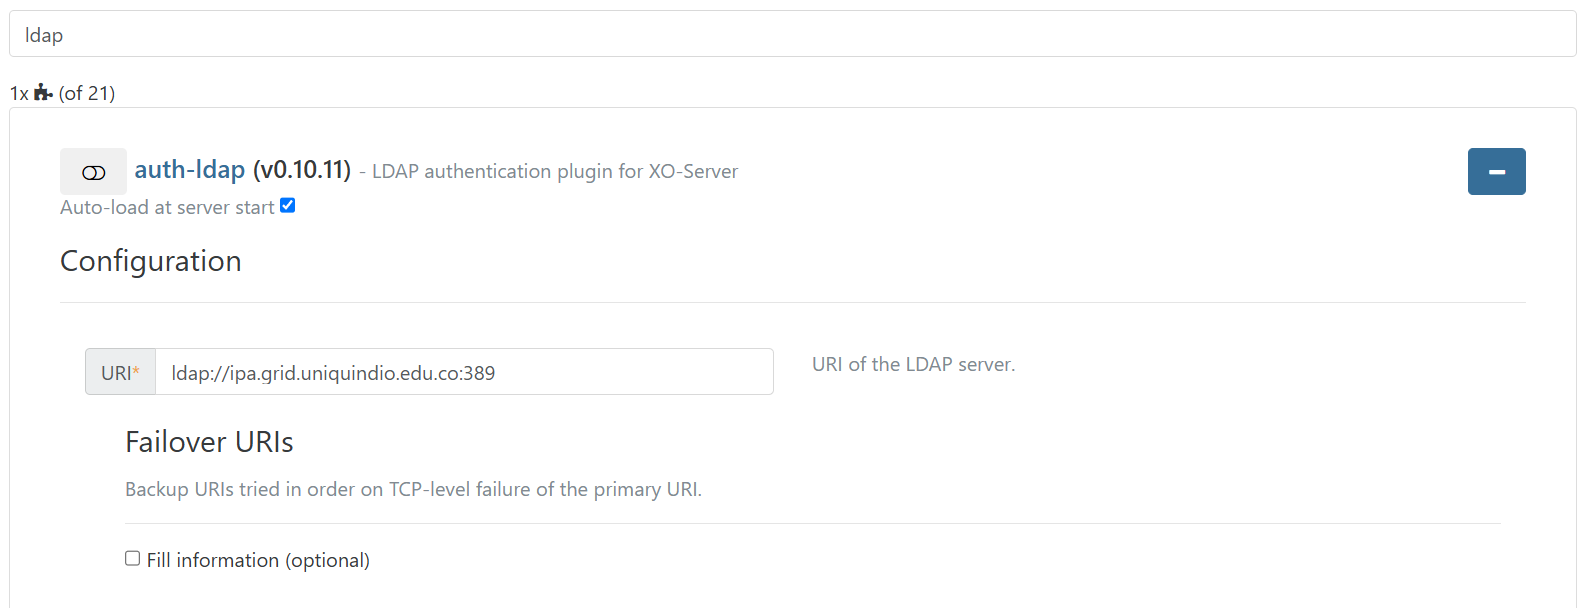
\includegraphics[width=0.8\textwidth]{mainmatter/II-desarrollo-metodologico/implementacion/imagenes/configuracion-uri-ldap-xen-orchestra.png}
	\caption{Configuración de la \acs{URI} del servidor \acs{LDAP} en el complemento de Xen Orchestra}
	\label{fig:configuracion-uri-ldap-xen-orchestra}
\end{figure}

Posteriormente, se configuraron los parámetros relacionados con la seguridad de la conexión y el ámbito de búsqueda dentro del directorio. En primer lugar, se estableció la ruta /home/node/ca.crt correspondiente al certificado de la autoridad certificadora de FreeIPA, el cual será utilizado para validar el certificado presentado por el servidor \ac{LDAP}. Para mantener la verificación de la identidad del servidor, se habilitó la opción Check certificate. Asimismo, se activó Use StartTLS, permitiendo que la conexión inicialmente establecida mediante \ac{LDAP} sea protegida mediante \ac{TLS}.

Finalmente, se definió como base del directorio el \ac{DN} \nolinkurl{dc=grid,dc=uniquindio,dc=edu,dc=co}. Este valor determina el punto de inicio dentro del árbol \ac{LDAP} a partir del cual el complemento realizará las búsquedas de usuarios y grupos. La combinación de estos parámetros permite establecer una conexión \ac{LDAP} cifrada y validar la identidad del servidor antes de realizar las consultas al directorio. La configuración del certificado, la seguridad \ac{TLS} y la base del directorio se observa en la \autoref{fig:configuracion-tls-base-xen-orchestra}.

\begin{figure}[H]
	\centering
	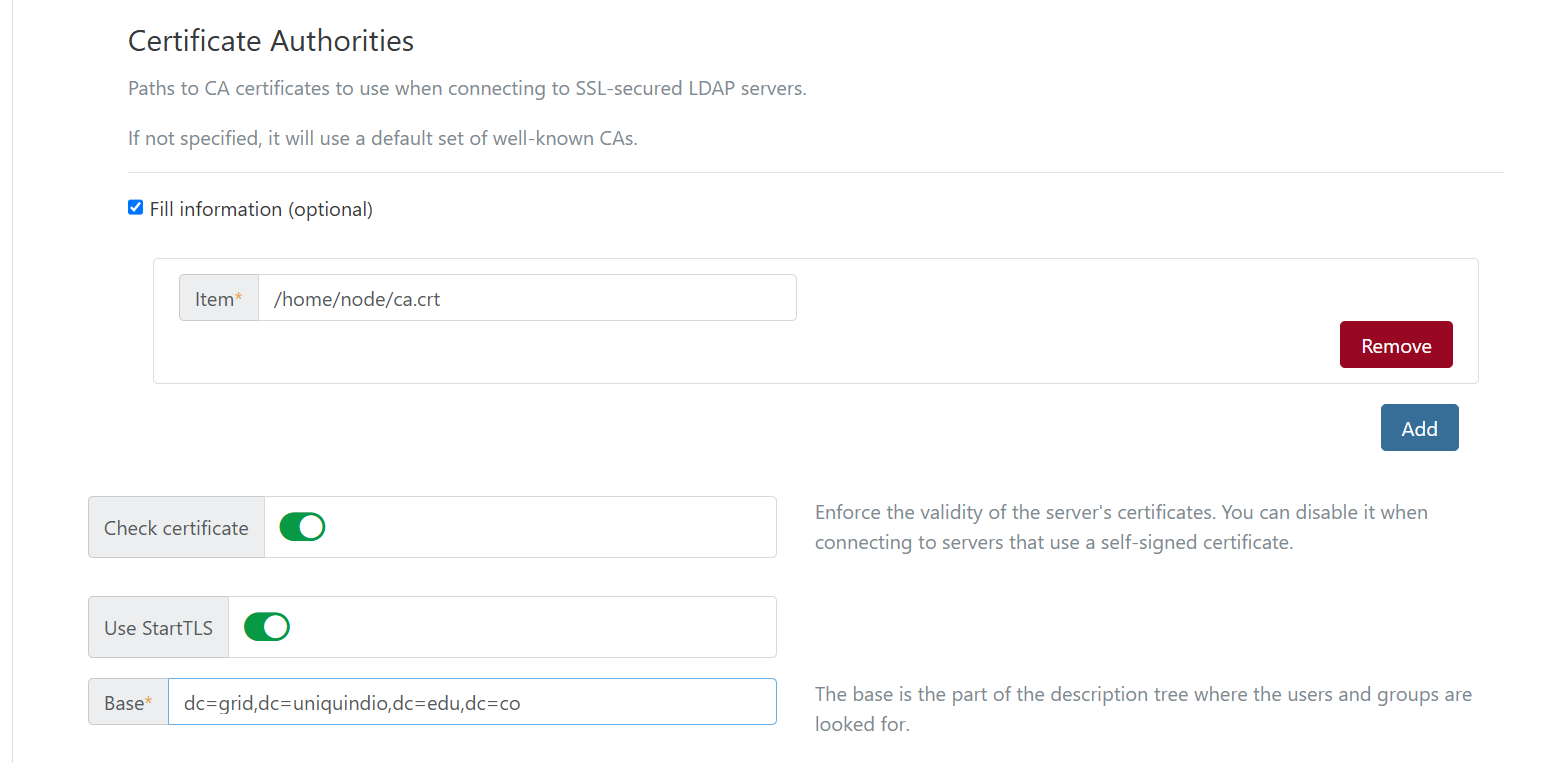
\includegraphics[width=0.8\textwidth]{mainmatter/II-desarrollo-metodologico/implementacion/imagenes/configuracion-tls-base-xen-orchestra.png}
	\caption{Configuración del certificado, seguridad \acs{TLS} y base del directorio \acs{LDAP} en Xen Orchestra}
	\label{fig:configuracion-tls-base-xen-orchestra}
\end{figure}

A continuación, se configuraron las credenciales que utilizará el complemento para realizar las consultas en el directorio \ac{LDAP} antes de localizar el registro correspondiente al usuario que intenta autenticarse. Para ello, se definió el \ac{DN} de la cuenta de servicio svc-xenorchestra, previamente creada para la integración con Xen Orchestra, junto con su respectiva contraseña. Esta cuenta permite realizar las búsquedas necesarias dentro del directorio sin utilizar las credenciales del usuario que posteriormente se autentica.

Adicionalmente, se configuró el filtro de usuario, mediante el cual se establece la condición que debe cumplir la cuenta para ser considerada durante el proceso de autenticación. En este caso, el filtro combina la identificación del usuario proporcionada por Xen Orchestra con su pertenencia al grupo xenorchestra, permitiendo que únicamente los usuarios autorizados para este servicio sean considerados por el complemento. La configuración de las credenciales y el filtro de búsqueda de usuarios se presenta en la \autoref{fig:configuracion-credenciales-filtro-xen-orchestra}.

\begin{figure}[H]
	\centering
	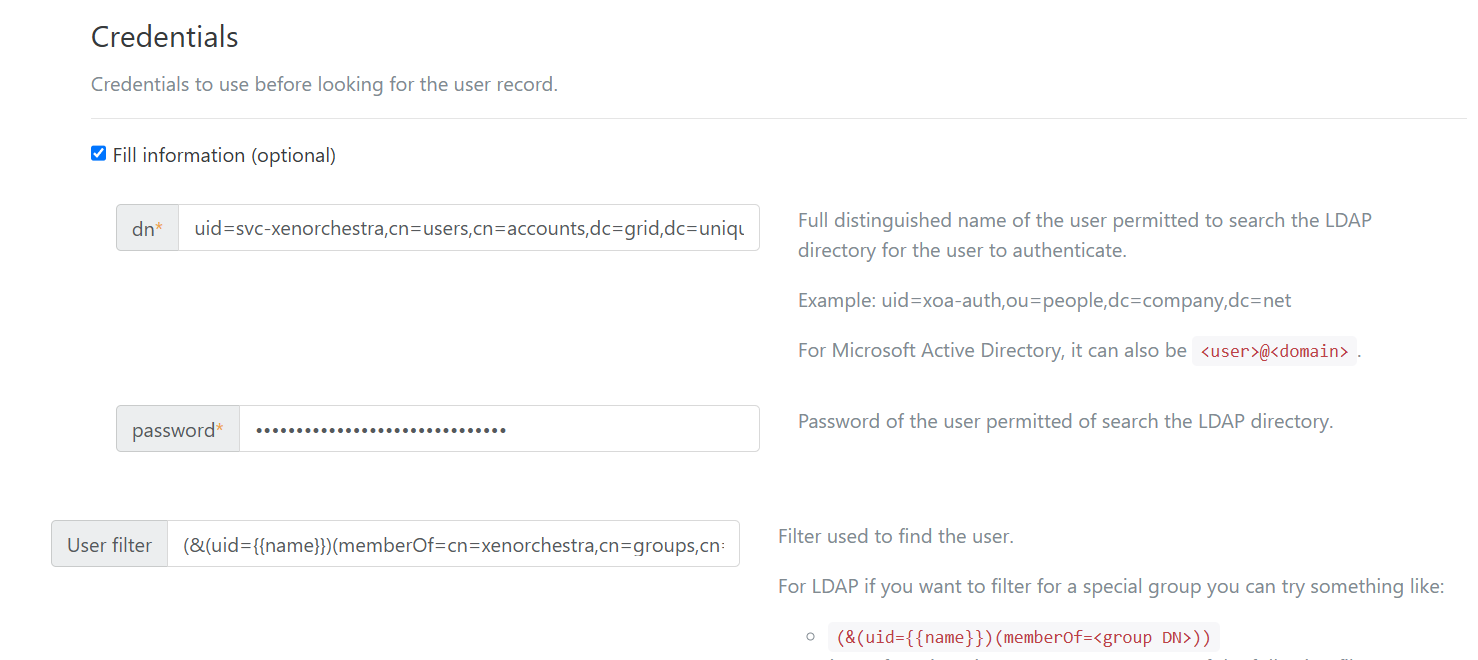
\includegraphics[width=0.8\textwidth]{mainmatter/II-desarrollo-metodologico/implementacion/imagenes/configuracion-credenciales-filtro-xen-orchestra.png}
	\caption{Configuración de las credenciales y filtro de búsqueda de usuarios \acs{LDAP} para Xen Orchestra}
	\label{fig:configuracion-credenciales-filtro-xen-orchestra}
\end{figure}

Finalmente, se configuró el atributo que permite identificar de forma única a los usuarios de \ac{LDAP} dentro de Xen Orchestra. Para este propósito, se estableció el atributo uid, utilizado para asociar cada cuenta del directorio con su correspondiente usuario en la plataforma. Asimismo, se mantuvieron sin configurar las opciones de sincronización de grupos y dominios adicionales, debido a que la integración implementada no requiere importar los grupos de FreeIPA directamente en Xen Orchestra ni utilizar dominios \ac{LDAP} adicionales.

Una vez definidos los parámetros necesarios, se procedió a guardar la configuración del complemento mediante la opción \textit{Save configuration}, dejando establecida la conexión entre Xen Orchestra y el servicio de directorio FreeIPA. Los parámetros finales de la configuración del complemento \ac{LDAP} y la opción para guardar la configuración se presentan en la \autoref{fig:configuracion-final-ldap-xen-orchestra}.

\begin{figure}[H]
	\centering
	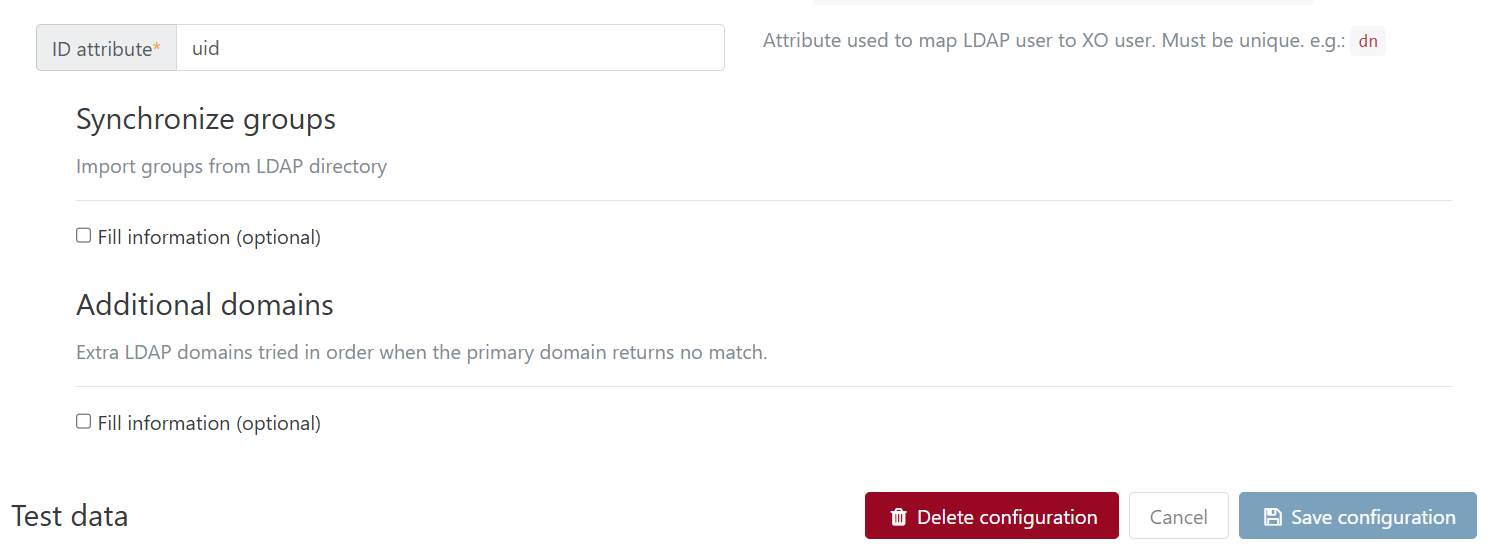
\includegraphics[width=0.8\textwidth]{mainmatter/II-desarrollo-metodologico/implementacion/imagenes/configuracion-final-ldap-xen-orchestra.png}
	\caption{Configuración final del complemento \acs{LDAP} en Xen Orchestra}
	\label{fig:configuracion-final-ldap-xen-orchestra}
\end{figure}

Finalmente, una vez completada la configuración del complemento, se procedió a activar el plugin \ac{LDAP} para poder realizar las pruebas de autenticación. Para ello, se utilizaron los datos de prueba disponibles en la sección \textit{Test data}, donde se ingresaron las credenciales de un usuario de FreeIPA y posteriormente se ejecutó la opción \textit{Test plugin}. Esta prueba permite comprobar el funcionamiento del complemento una vez habilitado y verificar que podía procesar correctamente las credenciales suministradas. Como resultado, Xen Orchestra mostró el mensaje \textit{“The test appears to be working”}, confirmando que la configuración realizada permitía establecer correctamente la comunicación y autenticación mediante \ac{LDAP}.

Los datos utilizados para la prueba se presentan en la \autoref{fig:datos-prueba-ldap-xen-orchestra}, mientras que el resultado satisfactorio obtenido se muestra en la \autoref{fig:resultado-prueba-ldap-xen-orchestra}.

\begin{figure}[H]
	\centering
	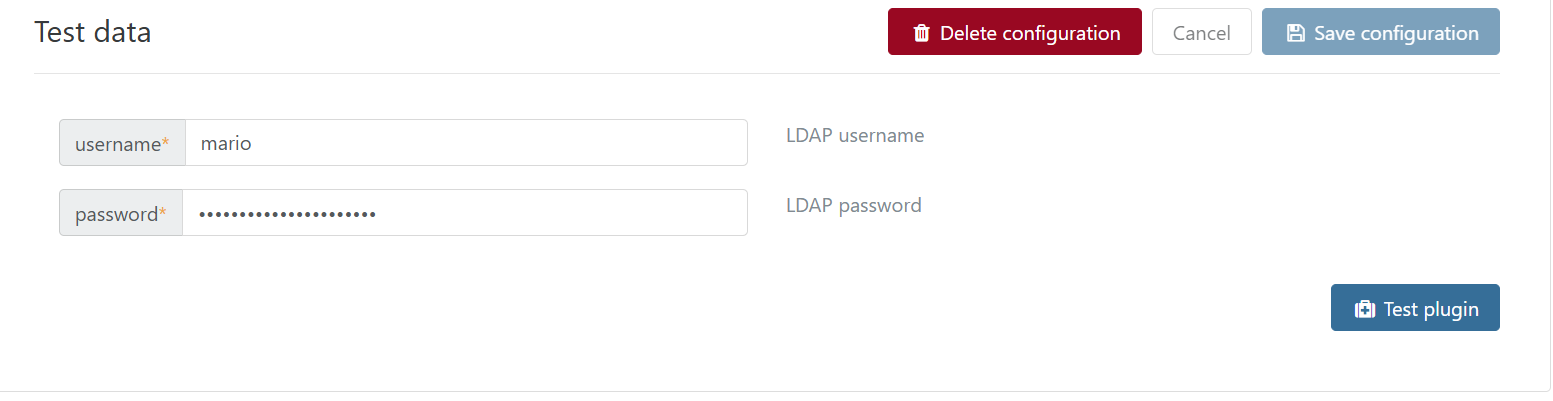
\includegraphics[width=0.8\textwidth]{mainmatter/II-desarrollo-metodologico/implementacion/imagenes/datos-prueba-ldap-xen-orchestra.png}
	\caption{Datos utilizados para la prueba del complemento \acs{LDAP} en Xen Orchestra}
	\label{fig:datos-prueba-ldap-xen-orchestra}
\end{figure}

\begin{figure}[H]
	\centering
	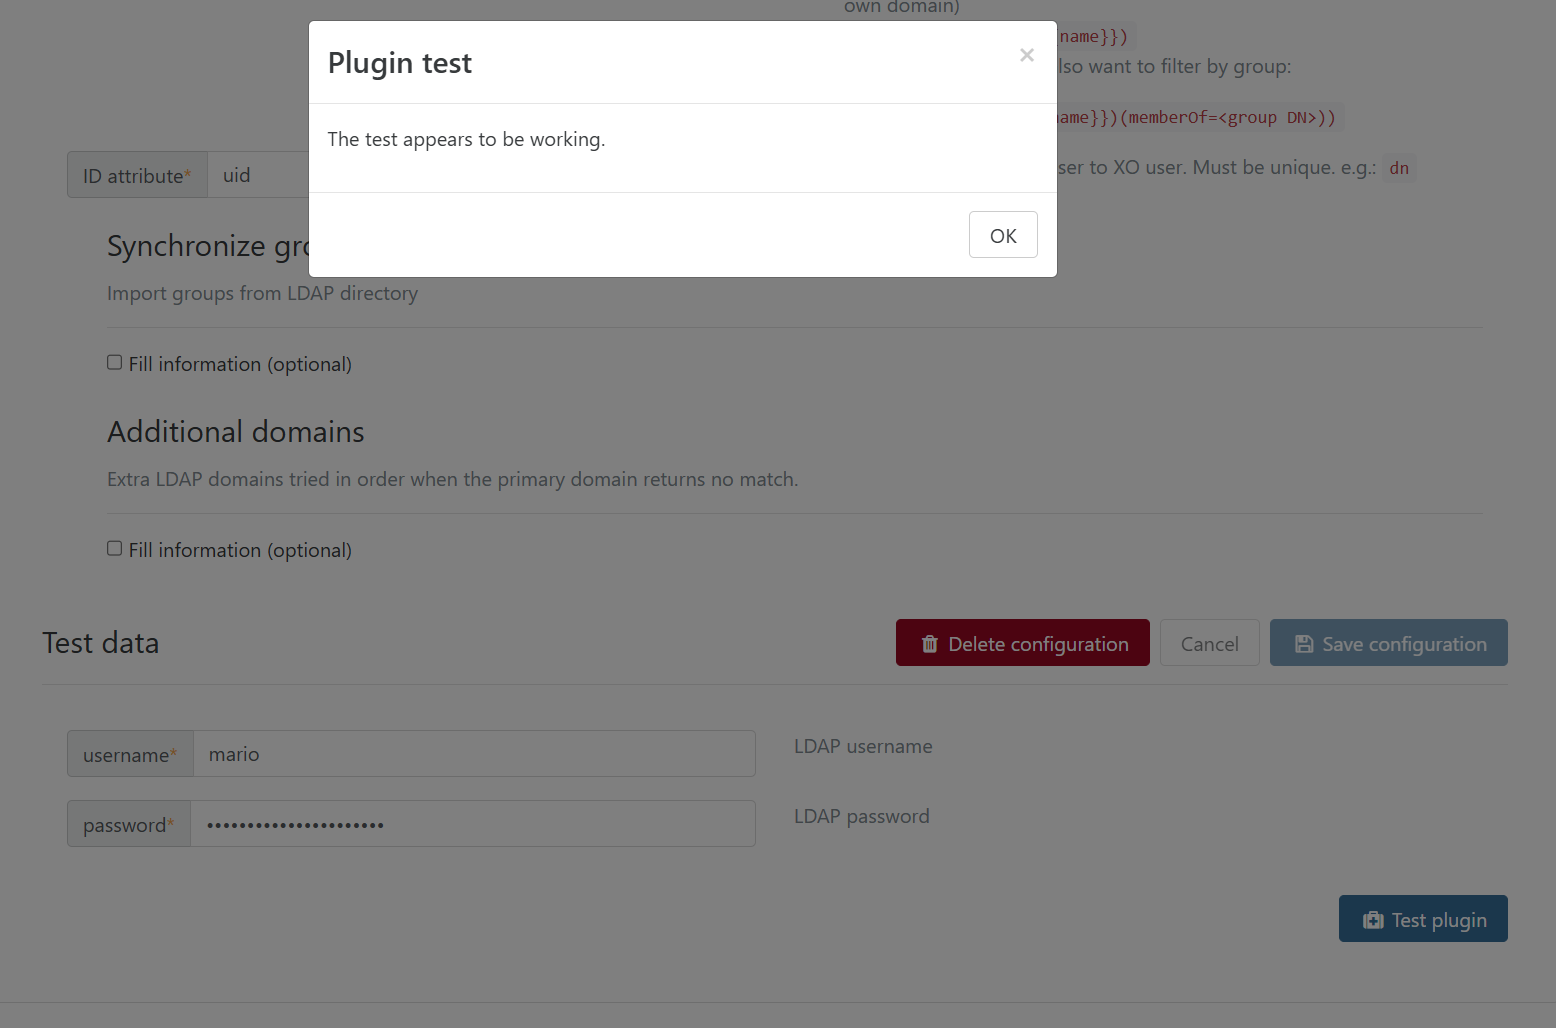
\includegraphics[width=0.8\textwidth]{mainmatter/II-desarrollo-metodologico/implementacion/imagenes/resultado-prueba-ldap-xen-orchestra.png}
	\caption{Resultado de la prueba de funcionamiento del complemento \acs{LDAP} en Xen Orchestra}
	\label{fig:resultado-prueba-ldap-xen-orchestra}
\end{figure}

